\documentclass[11pt,a4paper,twoside]{report}
    \usepackage{a4wide}
    \usepackage{epsfig}
    \usepackage{amsmath}
    \usepackage{tabu}
    \usepackage{amsfonts}
    \usepackage{latexsym}
    \usepackage[utf8]{inputenc}
    \usepackage{listings}
    \usepackage{color}
    \usepackage{titlesec}    
    \usepackage{enumitem}
    \usepackage[catalan]{babel}
    \usepackage{newunicodechar}
    \usepackage{graphicx}
    \usepackage{subcaption}
    \usepackage{float}
    \usepackage{xcolor}
    \usepackage{pgf, tikz}
    \usepackage{listings}
    \usepackage{booktabs}
    \usepackage[sorting=none]{biblatex}
    \usepackage{eurosym}
    \usepackage[figuresleft]{rotating}
    \usepackage{mathtools}
    \usepackage{pdfpages}
    \usepackage{multirow}
    \usepackage{array, multirow}

    \addbibresource{bibliography.bib}
    \bibliography{bibliography}
    
  \setcounter{tocdepth}{2}
  \setcounter{secnumdepth}{4}
  
  \newunicodechar{Ŀ}{\L.}
  \newunicodechar{ŀ}{\l.}
  \definecolor{dkgreen}{rgb}{0,0.6,0}
  \definecolor{gray}{rgb}{0.5,0.5,0.5}
  \definecolor{mauve}{rgb}{0.58,0,0.82}
  
  \DeclareSourcemap{
  \maps[datatype=bibtex]{
    \map{
      \step[fieldsource=howpublished, match=\regexp{\A\\url\{(.+ | $)\}\Z}, final]
      \step[fieldset=url, fieldvalue={$1}]
      \step[fieldset=howpublished, null]
    }
  }
}
\definecolor{maroon}{rgb}{0.5,0,0}
\definecolor{darkgreen}{rgb}{0,0.5,0}
\lstdefinelanguage{XML}
{
  basicstyle=\ttfamily,
  morestring=[s]{"}{"},
  morecomment=[s]{?}{?},
  morecomment=[s]{!--}{--},
  commentstyle=\color{darkgreen},
  moredelim=[s][\color{black}]{>}{<},
  moredelim=[s][\color{red}]{\ }{=},
  stringstyle=\color{blue},
  identifierstyle=\color{maroon}
}

  \usepackage{hyperref}
  \hypersetup{
    colorlinks=false, %set true if you want colored links
    linktoc=all,     %set to all if you want both sections and subsections linked
    linkcolor=blue,  %choose some color if you want links to stand out
  }
  
  \setlength{\footskip}{50pt}
  \setlength{\parindent}{0cm} \setlength{\oddsidemargin}{-0.5cm} \setlength{\evensidemargin}{-0.5cm}
  \setlength{\textwidth}{17cm} \setlength{\textheight}{23cm} \setlength{\topmargin}{-1.5cm} \addtolength{\parskip}{2ex}
  \setlength{\headsep}{1.5cm}
  
  \renewcommand{\contentsname}{Continguts}
  \setcounter{chapter}{0}
  % \titleformat{\chapter}[display]
  % {\normalfont\bfseries}{}{0pt}{\Large}
  \titleformat{\chapter}[block]
  {\normalfont\LARGE\bfseries}{\thechapter.}{1em}{\LARGE}
  \titleformat{\section}[block]
  {\normalfont\Large\bfseries}{\thesection.}{1em}{\Large}
  
  \begin{document}
  \begin{titlepage}
    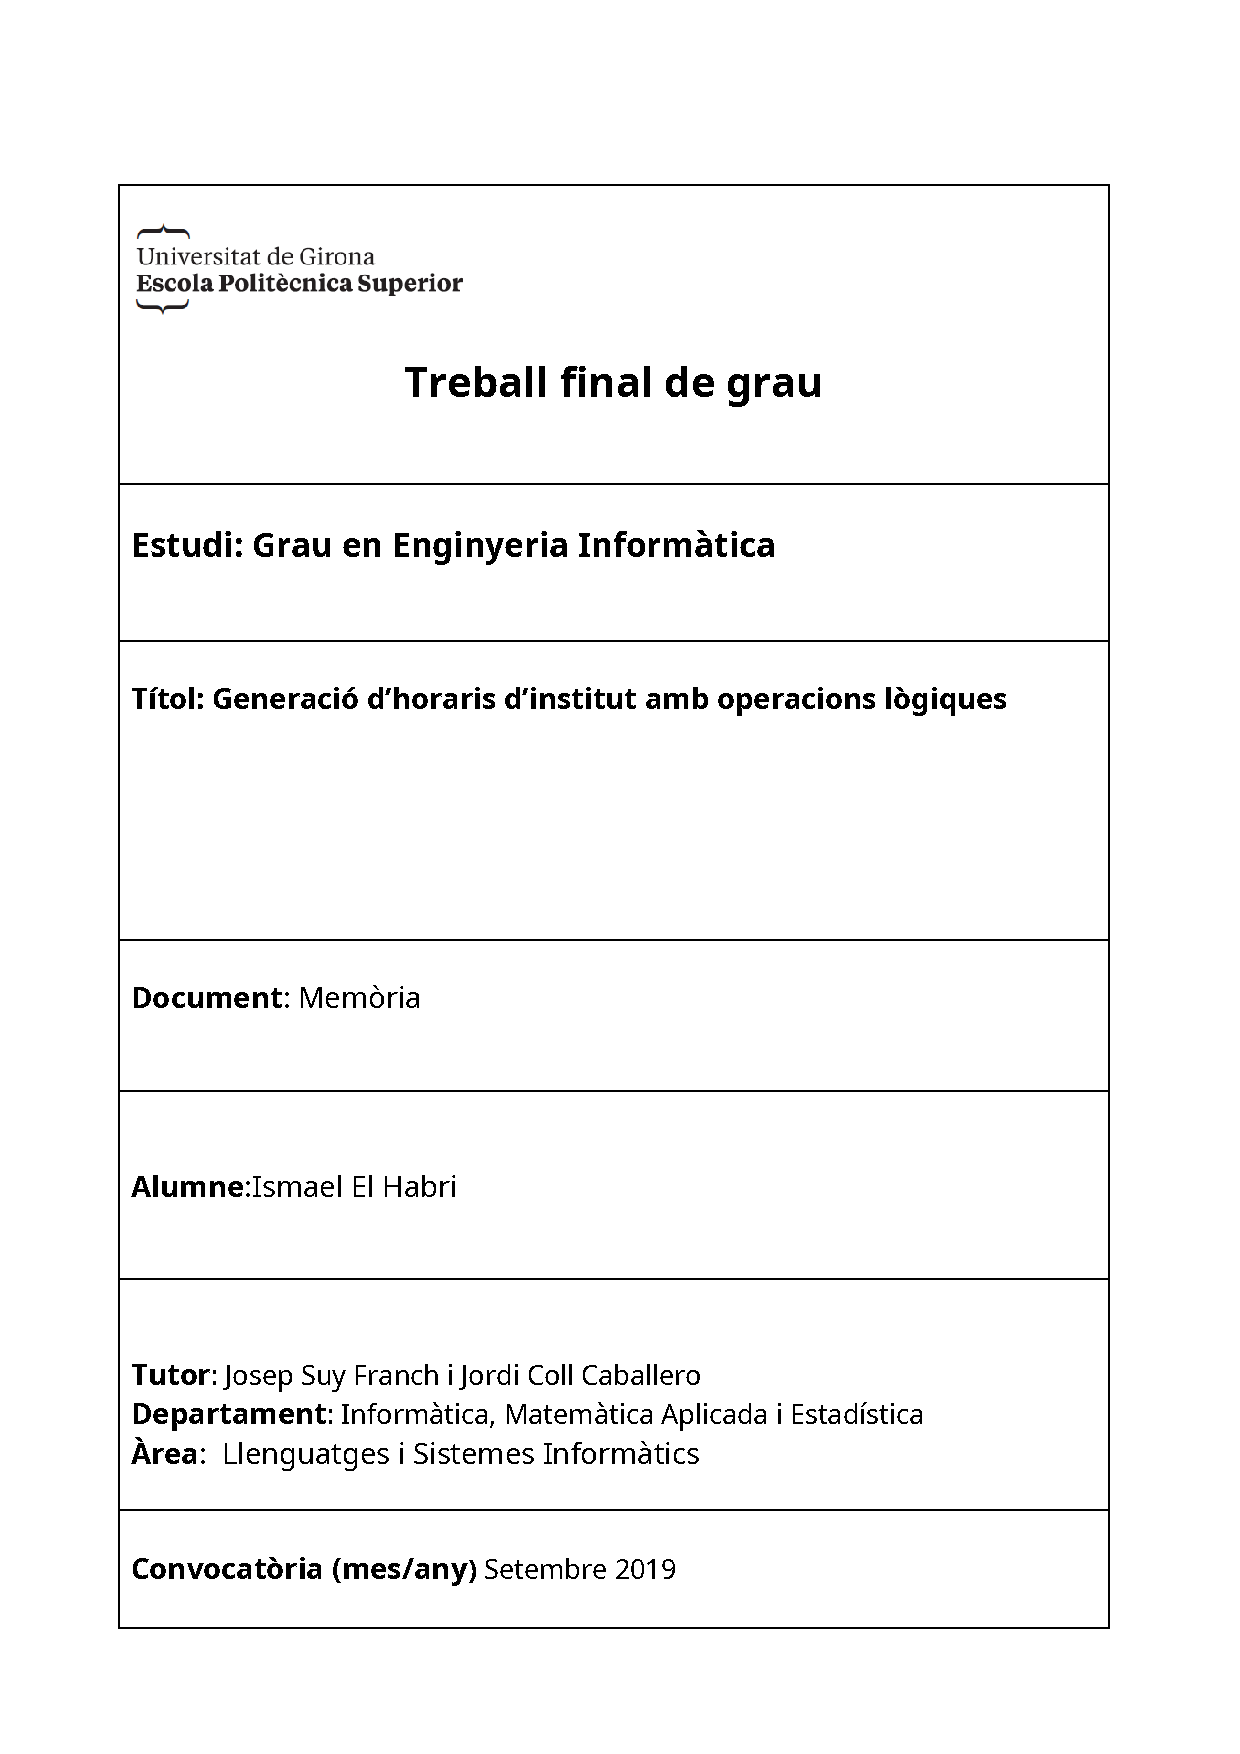
\includepdf[pages=1]{portada.pdf}
  \end{titlepage}


  \shipout\null
  \tableofcontents
  
  \chapter{Introducció, motivacions, propòsit i objectius}
  
  % \section{Introducció}
  % \section{Motivacions}
  % \section{Propòsit}
  % \section{Objectius}

  La confecció d'horaris és un problema recurrent amb el qual es troben els instituts que amaga una alta combinatòria, 
  dificultant-ne molt la seva elaboració manual donat que s'han de prendre moltíssimes decisions a cegues,
  fa que sigui molt probable cometre errors en la confecció. En aquesta situació, amb l'aparició dels computadors molts instituts varen decidir ajudar-se en aquesta tasca utilitzant eines informàtiques capaces 
  d'explorar grans quantitats de combinacions per segon. No obstant a això, 
  amb aquelles primeres eines sguim tenint molts problemes per generar horaris viables i normalment donaven resultats que
   eren de qualitat baixa i requerien un refinament posterior que s'havia de fer de forma manual.
  
  El HSTT (High School TimeTabling) consisteix en la solució de forma automàtica d'aquest problema d'alta complexitat (NP). 
  Així doncs, el que s'intenta és la configuració automàtica d'horaris d'institut partint d'una sèrie de recursos 
  (per exemple: aules, professors, assignatures, grups) i repartir-los de manera que sigui viable i tenint en compte 
  de manera total o parcial les preferències del professorat respecte a horaris, continuïtat, grups, etc. 
  Tot això, fa que el problema sigui molt difícil de resoldre a causa del gran nombre de combinacions possibles entre els diferents recursos.
  
  Afegint dificultat al problema, depenguen del país del qual estiguem parlant existeixen una gran diversitat de requisits propis, degut a les característiques pròpies del sistema d'estudis secundaris de cada lloc.

  A causa de tot el mencionat encara no existeix cap eina capaç 
  de trobar una solució òptima al problema de manera determinista en un temps raonable. 
  Encara que s'ha avançat molt en la resolució de problemes d'aquest tipus i actualment
  costa trobar instituts que optin per fer els horaris de forma manual.

  
  Els objectius d'aquest treball són els següents:
  \begin{itemize}
    \item Aprofundir sobre el problema de la generació d'horaris en sí i sobre els problemes de satisfacció de restriccions en general i les tècniques que s'utilitzen per resoldre'ls, com ara, SAT i les seves diverses extensions.
    \item Desenvolupar un generador d'horaris automàtic utilitzant les tècniques estudiades anteriorment. 
    Aprofitant les eines relacionades que s'han desenvolupat recentment pel grup de recerca Lògica i Programació, 
    s'intentarà resoldre el problema en un temps raonable i intentar trobar la millor solució possible. 
    Això que es preveu molt complicada d'aconseguir en un temps raonable en les instàncies grosses.
    
  \end{itemize}
  
  \section{Grup de recerca Lògica i Programació}
  Aquest treball s'emmarca dins del grup de recerca de Lògica i Programació de l'àmbit d'àrea tècnica de la Universitat de Girona.

  El grup basa la seva recerca en l'estudi de satisfactibilitat de fórmules proposicionals booleanes (SAT) 
  i Satisfiability Modulo Theories (SMT) i les seves
  aplicacions per a la resolució de problemes combinatoris com ara problemes de \textit{scheduling} i \textit{planning} 
  . El grup ha arribat a utilitzar amb èxit tècniques innovadores en altres àmbits com
  pot ser: els problemes de \textit{scheduling} i \textit{planning}.

  Durant l'elaboració del treball he rebut ajuda i assessorament dels membres del grup, incloent els meus tutors de projecte, el Dr. Josep Suy i el Dr. Jordi Coll, qui també en formen part.

  \section{Estructura del Treball}
  A continuació s'exposa l'estructura d'aquest document: 
  \begin{enumerate}
    \item Introducció, motivacions, propòsit i objectius: Situa el marc del projecte, explica les raons per les quals s'ha escollit el treball i en defineix els objectius.
    \item Estudi de viabilitat: Justifica la capacitat de fer el projecte
    \item Metodologia i Planificació: Tot i que a la guia van separats, s'ha decidit ajuntar-los per la gran relació que tenen entre ells. En aquest apartat s'exposa la metodologia que s'ha seguit a l'hora d'implementar el projecte i es defineix l'estratègia seguida per arribar als objectius.
    \item Marc de treball i conceptes previs: S'exposa el treball previ realitzat sobre el problema, i els coneixements necessaris per a la implementació del programa.
    \item Requisits del sistema: Requisits funcionals i no funcionals que ha de complir el sistema.
    \item Anàlisi i disseny del sistema: Descripció del maquinari i programari utilitzat durant el desenvolupament del projecte.
    \item Implementació i proves: Es detalla la implementació del programa, els problemes que han aparegut i les solucions que s'han donat a aquests.
    \item Resultats: Detalla els resultats obtinguts. L'apartat d'implantació que segons la guía donada va aquí, s'ha descartat posat que en aquest treball no té l'objectiu d'implantar res.
    \item Conclusions: Conclusió del projecte i els resultats
    \item Treball futur: Possibles ampliacions, millores o treballs futurs que es poden realitzar.
    \item Bibliografia: Referències utilitzades per desenvolupar el projecte.
    \item Manual d'usuari i insta\l.lació: Especifica les passes a seguir per utilitzar el sistema creat en un ordinador.

  \end{enumerate}

%   La introducció serveix per situar el marc del projecte. Aquesta primera etapa implica
% establir les raons que justificaven el desenvolupament del projecte i el que se
% n’esperava obtenir. Aquest propòsit és, per naturalesa, una idea molt ampla.
% Pel contrari, els objectius identifiquen les fites específiques que l’estudiant esperava
% assolir en el seu camí cap al propòsit últim del projecte. Els objectius són més
% precisos que el propòsit general. A partir d’aquesta informació s’ha de comprendre
% millor el projecte, identificar l’entorn on es desenvolupa i entendre millor quina és la
% feina que ha calgut fer.
% En l’apartat anterior, cal precisar i no confondre entre el que són els objectius del
% projecte i els requisits del producte final (aplicació, sistema de maquinari,
% algorismes...).
% En cas que el projecte es desenvolupi en un entorn consolidat (grup de recerca,
% empresa, institució...), aquest apartat pot incloure una descripció de l’entorn en el
% qual es desenvolupa el projecte, així com una especificació del punt de partida del
% projecte. També cal deixar clar en aquest punt quina és l’aportació del P/TFC en
% relació amb el punt de partida.
% En aquest apartat l’estudiant també ha de justificar els apartats de la memòria
% afegits, suprimits o canviats d’ordre respecte del que descriu aquest document.
  \chapter{Estudi de viabilitat}

  \section{Viabilitat tècnica}

  Per tal de realitzar aquest projecte farà el software necessari per poder tractar un fitxer XML, codificar una instància del problema en C++ i resoldre-la amb un \textit{solver} SAT o d'alguna extensió de SAT. 
  Abans de iniciar el projecte, s'ha comprovat l'existència d'aquest software i que aquest estigués disponible de forma gratuïta, de fet, tot el software que s'utilitzi en aquest projecte serà de codi obert.

  Per part dels requisits de maquinari, tot i que HSTT és un problema dur, 
  després de veure el treball previ realitzat en aquest mateix problema i d'altres de característiques semblants, s'ha determinat que la meva màquina d'ús diari és més que suficient per a tal de realitzar el desenvolupament del generador d'horaris.

  Pel que fa a l'habilitat de desenvolupar aquest treball s'ha determinat que era possible gràcies al fet que
  el grup de recerca Lògica i Programació ha treballat i aconseguit solucionar problemes semblants de forma exitosa utilitzant tècniques innovadores. 
  Utilitzant els avenços fets pel grup s'ha decidit que es podria desenvolupar el treball en el marc de temps desitjat.



  \section{Viabilitat econòmica}
  
  Gràcies a que tot el software utilitzat és gratuït, lliure i de codi obert, i que el codi que el grup de recerca m'ha cedit també ha estat gratuït. Per part del maquinari, només s'ha utilitzat el que ja tenia amb anterioritat, així que per aquesta banda tampoc ha suposat cap cost.
  Així doncs, aquest projecte no s'ha requerit de cap inversió ni despesa econòmica. 
  Així doncs l'únic cost que ha suposat aquest treball han estat el temps necessari per fer-lo i les ganes que se li han hagut de ficar. 


  \subsection{Pressupost}
  Tot i que, com s'ha explicat anteriorment, el desenvolupament d'aquest treball no té cost, s'ha decidit fer una simulació del que costaria contractar un programador per fer el treball.
  
  \begin{center}
    \begin{tabular}{|| c | c | c | c||} 
    \hline
     & \euro/h & Hores & Cost \\ [0.5ex] 
    \hline\hline
    Programador & 14 & 260 & 2520 \\ [1ex] 
    \hline
   \end{tabular}
   \end{center}

   A part també s'han de tenir en compte el maquinari utilitzat:
   \begin{center}
    \begin{tabular}{|| c | c | c | c||} 
    \hline
     & Cost Total & Hores & \euro/h \\ [0.5ex] 
    \hline\hline
    Ordinador Principal & 828 & 240 & 3.45 \\ [1ex] 
    Ordinador Portatil Secundari & 200 & 20 & 10 \\ [1ex] 
    \hline\hline
    Total & 1028 & 260 & 3.95 \\


    \hline
   \end{tabular}
   \end{center}


   També cal tenir en compte que els tutors del treball m'han ajudat molt, i han dedicat part del seu temps en les reunions, intercanvis de mails i conversacions que s'han tingut sobre el treball.
   \begin{center}
    \begin{tabular}{|| c | c ||} 
    \hline
     & Hores \\ [0.5ex] 
    \hline\hline
    Josep Suy & 30 \\ [1ex] 
    Jordi Coll & 20 \\ [1ex] 
    \hline
   \end{tabular}
   \end{center}
  % preguntar suy
  %==================
  % Cal justificar quins són els paràmetres que feien possible el desenvolupament del
  % projecte. Aquest punt pot incloure els recursos necessaris per desenvolupar el
  % projecte, els pressupostos inicials, la viabilitat tecnològica i/o econòmica, els
  % recursos humans, etc.
  %

  \chapter{Metodologia i Planificació}
  \section{Metodologia}
  La part més important i grossa d'aquest treball és la creació d'un generador automàtic d'horaris utilitzant les eines oferides pel grup de recerca. 
  Primer caldrà estudiar el problema (HSTT) i la seva duresa, per poder ser capaç d'entendre el què estem treballant.
  Des de aquí es procedirà a la implementació del programa, utilitzant la API SMT creada pel Dr. Jordi Coll, el qual es membre del grup de recerca de Lògica i Programació del departament d'Informàtica, Matemàtica Aplicada i Estadística.
  Aquesta API ens estalviarà la codificació de les restriccions de cardinalitat i les restriccions pseudo-booleanes, 
  a part d'oferir-nos una interfície senzilla per poder implementar el model en diferents \textit{encodings} i múltiples opcions.

  Després de fer un estudi preliminar del problema i el treball previ respecte aquest, la metodologia de treball que s'ha seguit ha estat la d'entregues periòdiques. 
  Consistint a fer una reunió amb els tutors per decidir el pròxim pas del treball i jo dedicar-me durant un temps a fer aquest pas. Després d'aquest temps es convoca una altra reunió on es valora el treball fet i es decideix com seguir. 
  Des d'aquí es va repetint fins a acabar el projecte.

  El model de desenvolupament que s'ha triat en aquest treball ha estat el model de prototips (o prototipatge), 
  que consisteix a crear, com el nom indica, prototips del programari que es pretén crear, és a dir, versions incompletes del software que s'està desenvolupant.
  Generalment, un prototip només compleix alguns dels requeriments del sistema i pot no tenir res a veure amb el producte final. Aquest model presenta diferents beneficis:
  \begin{itemize}
    \item Permet obtenir \textit{feedback} molt aviat en les etapes de desenvolupament.
    \item Augmenta la precisió de les estimacions de temps de dedicació a la implementació de les funcionalitats. 
    \item Permet que els desenvolupadors se centrin en treballar en les parts del sistema que comprenen i no haver d'implementar tot el sistema de cop.
  \end{itemize}



  %1 - estudiar el problema
  %2 - fer el parser
  %3 - testejar el parser
  %4 - estudi yices
  %5 - estudi api smt jordi coll
  %6 - fer model
  %7 - testing model
  %8 - proves diferents encodings de les cardinality constraints
  %9 - millora format output
  %10 - si cal, confeccio model
  \section{Planificació}

  Com s'ha dit en l'apartat anterior primer caldrà estudiar el problema HSTT i la seva duresa. 
  Després es procedirà amb el disseny i la implementació del generador. Primer caldrà dissenyar implementar i depurar un \textit{parser} pels fitxers. En aquest pas també cal pensar i implementar en quina estructura es guardaran aquestes dades i com es transferiran en el model que es codificarà posteriorment. 

  Al tenir el \textit{parser} i l'estructura de dades enllestits caldrà començar a estudiar com funciona la API per C++ del Yices i 
  posteriorment la API SMT del Dr. Jordi Coll. Això ens permetrà començar a dissenyar, codificar i testejar el model, que és el següent pas del treball. 
  Al tenir enllestit el model, es faran les proves de rendiment amb diferents límits d'optimització i diferents \textit{encodings} de les restriccions de cardinalitat.
  Finalment s'implementarà una forma maca i llegible de mostrar els horaris generats.
  
  Amb això el generador es donarà per acabat i es passarà a la confecció de la memòria del treball. 
  A continuació un diagrama de Gantt mostrant la planificació feta.

  %% diagrama de gantt...

  %% CAL AMPLIAR

  \begin{figure}
    \centering
    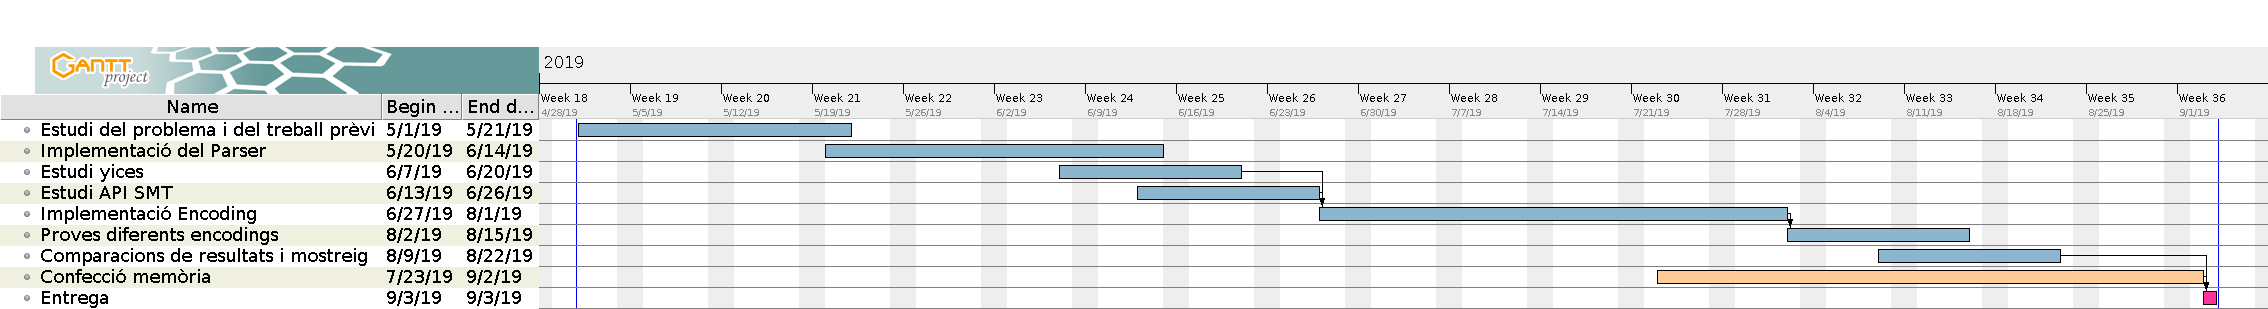
\includegraphics[angle=90,origin=c,height=0.58\textheight]{Diagrames/gantt1.png} 
    \caption{Diagrama de Gantt amb la planificació de treball del projecte}
    \label{fig:Gantt}
  \end{figure}




  \chapter{Marc de treball i conceptes prèvis}
  \section{Marc de treball}
    Com s'ha mencionat en la introducció aquest treball s'emmarca dins del grup de recerca de Lògica i Programació (LAP) del departament d'Informàtica, Matemàtica Aplicada i Estadística (IMAE) de la Universitat de Girona. 
    En el treball s'utilitzaran les eines desenvolupades recentment en el grup de recerca, per ser exactes, la API SMT feta en C++ pel Dr. Jordi Coll. 
    Aquesta API permet codificar problemes SAT, MaxSAT i SMT per a diferents \textit{solvers} de forma transparent a aquest i té implementades les diferents restriccions de cardinalitat i pseudo-booleanes en les diferents possibles codificacions. 
    També inclou diferents algoritmes d'optimització implementats.

    La resta del treball previ seria el treball final de grau fet el 2015 per en Cristòfor Nogueira, el qual també consisteix en la confecció d'horaris d'institut \cite{treballCristo}.
    %nose seguir  
    %s'ha de mencionar el treball den cristofol, probablament, 

  \section{Definició del problema}
    El problema que es treballa és el de la confecció d'horaris per a institut (HSTT de \textit{High School Time Tables}). 
    Aquest consisteix en assignar a cada assignatura que es fa en un centre l'espai de temps en què s'impartirà i el conjunt de recursos que utilitzarà. 
    Els recursos normalment seran professors i aules, però es contemplen altres possibles necessitats especials de cada centre, per això es generalitza.

    La duresa d'aquest problema es troba en assignar un espai de temps per a cada assignatura donant-li els recursos que necessita sense violar cap restricció que aquests tinguin, 
    com podria ser no fer dues assignatures a la vegada en la mateixa aula, o sigui, que en realitzar-se l'assignatura tots els seus recursos estiguin disponibles.  
    De la mateixa manera es poden imposar diverses restriccions de naturaleses diferents i amb cada una s'aniran reduint les possibles combinacions vàlides i fent més i més difícil la generació de l'horari.
    \subsection{Estudi de duresa}

    

    \subsubsection{Incís en la teoria de la computació}
    Abans de procedir a l'estudi de la duresa del problema HSTT, caldrà explicar els següents conceptes de la teoria de la computació: 
    \paragraph*{Problemes decidibles i indecidibles}

    Un problema decidible és aquell pel qual existeix una màquina de Turing que para en totes les entrades possibles amb una resposta: sí o no. Aquests problemes també són coneguts com a Turing Decidibles. 
    Així doncs, un problema decidible és aquell pel qual sempre podrem construir un algorisme que sempre respon el problema.
    
    Un problema pot ser semi-decidible, això passa quan una màquina de Turing quan l'entrada és acceptada, però es pot penjar o es pot parar quan l'entrada es rebutja. Aquests problemes també són referits com a Turing Reconeixibles.
    
    Un problema indecidible és aquell pel qual no podem construir un algorisme que resolgui el problema en temps finit. Aquests problemes poden ser parcialment decidibles, però sempre hi haurà una condició que portarà la màquina de Turing a bucle infinit.


    \paragraph*{P, NP i NP-Completesa}
    \begin{itemize}
      \item \textbf{P: }És el conjunt de problemes que poden ser resolts en temps polinòmic amb una màquina de Turing determinista. 
      \item \textbf{NP: }És el conjunt de problemes que poden ser resolts en temps polinòmic amb una màquina de Turing no determinista. 
      \item \textbf{NP-Complet: }És el conjunt de problemes més durs en el conjunt NP. Un problema C és NP-Complet si C és NP i tot problema NP és reductible a C.
      \item \textbf{NP-Hard: }És el conjunt de problemes als quals es pot reduir tot problema NP. O sigui, un problema C és NP-Hard si tot problema NP és reductible a C. 
      \item \textbf{Reducció: }Si tenim dos problemes $L_1$ i $L_2$  i tenim un algoritme $A_2$ que resol $L_2$. Reduir $L_1$ a $L_2$ és transformar el problema $L_1$ a $L_2$ així poder utilitzar el algoritme $A_2$ per resoldre el problema, creant així un algoritme $A_1$ amb l'estructura que es pot veure en la figura \ref{fig:reduccio}
      \begin{figure}[ht!]
        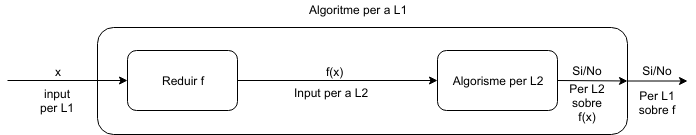
\includegraphics[width=\textwidth]{Diagrames/Reduccio.png}
        \caption{Esquema de Reducció}
        \label{fig:reduccio}
      \end{figure}
      
    \end{itemize}

    \subsubsection{Duresa de HSTT}
    El problema HSTT és clarament decidible i, posat que comprovar si una solució satisfà totes les restriccions imposades és d'ordre polinòmic, aquest pertany al conjunt de problemes NP.
    
    \paragraph*{NP-Completesa de HSTT} ~\\

    Es pot demostrar la NP-Completesa del problema HSTT reduint un problema NP-Complet conegut a HSTT, en aquest cas, el problema de la motxilla\cite{wiki:bin}, d'acord amb la demostració proposada per B. Cooper i J.H. Kingston \cite{complexityHSTT}.

    Una de les fonts de la duresa del problema ve a l'hora de gestionar els recursos de manera coherent. Així que al confeccionar un horari serà d'interès mantenir el nombre d'incoherències per sota un llindar. 
    Les instàncies HSTT acostumen a tenir com a mínim un tipus de recurs que compleix aquestes premisses. 
    En cas de que no en tinguin, és possible realitzar una transformació binària per arribar a aquesta formulació, 
    ja que tots els recursos poden atendre a un nombre limitat d'assignatures de manera simultània i totes les instàncies disposen d'un nombre limitat de recursos. Per tant, i per simplificar, considerarem només un únic recurs, de disponibilitat limitada. També considerarem que un recurs només pot atendre a una assignatura alhora.

    Diem que dues assignatures són incoherents si comparteixen algun espai de temps. És a dir, si se superposen. Com que els recursos són limitats interessa limitar el nombre de superposicions. Utilitzarem una codificació del problema de la motxilla per representar aquesta situació.

    El problema de la motxilla consisteix en determinar si un conjunt d'ítems $U = \{u_1, u_2, ..., u_n\}$, cadascun amb un pes associat $w_i$, es poden co\l.locar en un conjunt de motxilles $B = \{b_1, b_2, ..., b_m\}$, 
    cadascuna amb una capacitat màxima $c_i$ de manera que cap motxilla sobreexcedeixi la seva capacitat.

    Transformem el problema de la motxilla al següent problema HSTT: 
    \[
        Times = \{t_1,1, ..., t_n,m\}
    \]\[
        Events = X \cup Y, X = \{x_1, ..., x_n\} Y = \{y_1, ..., y_m\}
    \]

    De manera que: 
    \begin{itemize}
      \item A cada $x_i$ se li han d'assignar tants espais de temps com $w_i$.
      \item A cada $y_i$ se li han d'assignar tants espais de temps com $c_i$ i els corresponents a la motxilla que representen. És a dir, $y_i$ tindrà assignats els espais de temps $\{t_i,1 ... t_{i,c_i}\}$
    \end{itemize}
    
    El problema doncs, rau en determinar quins espais de temps s'assignen a cada $x_i$. 
    Suposem que aquest problema formulat com el de la motxilla té solució: $f: U \rightarrow B$ on el valor de retorn de $f$ és l'index de la motxilla on s'ha de co\l.locat l'ítem d'entrada. 
    Llavors, per cada assignatura $x_i$, escollim $w_i$ espais de temps, q no hagin estat escollits prèviament, del conjunt $S_k = \{t_k,1 ... t_{k, c_k}\}$, on $k = f(u_i)$. 
    És a dir, s'escullen tants espais de temps com el pes de l'ítem que representa de manera que no hi hagi solapaments entre els membres de X. Aquest procés és possible perquè $f$ ens garanteix que com a molt s'escolliran $c_k$ espais de temps de $S_k$. 
    Al final tenim que tots els events tenen assignats exactament $w_i$ espais de temps i cada $X_i$ se solapa amb un, i només un event de $Y$. Per tant, tenim que el nombre d'incoherències o superposicions és $n$.
    
    Ara, suposem que la instància que la instància HSTT que hem descrit genera una solució amb un nombre de solapaments $\leq n$. Sabem que com a mínim el nombre de superposicions ha de ser $\geq n$, ja que cada $x_i$ 
    s'ha de solapar com a mínim una vegada amb algun membre de Y. Per tant el nombre de solapaments de la solució generada per la instància HSTT ha de ser exactament n i cada event $x_i$ es solapa només una vegada amb un sol membre de $Y$.
    Podríem reimplementar, doncs, $f$ de manera que a partir de la solució obtinguda per la instància HSTT es limiti a esbrinar per cada event $u_i$, amb quint event $y_i$ es solapa, de manera que $f(u_i) =j$.

  \section{Format XHSTT}
  Un dels problemes que presenta HSTT és la complexitat que té representar una instància amb totes les possibles restriccions possibles. Per això s'ha optat utilitzar el format genèric per a representar les instàncies de HSTT anomenat XHSTT (de \textit{Xml-format High School TimeTabling}) utilitzat per HSEval\cite{xhstt}.
  Aquest format és obert i preveu l'addició d'elements i restriccions, així que en aquest treball només es tindran en compte un subconjunt d'ells.
  
  Aquest format utilitza quatre tipus de fills en les instancies:
  \begin{itemize}
    \item \textit{Times} pels espais de temps.
    \item \textit{Resources} pels recursos.
    \item \textit{Events} pels events, com ara assignatures.
    \item \textit{Constraitns} per les restriccions.
  \end{itemize}

  \subsection{Temps, Recursos i Events}
  \paragraph*{Temps}~\\
  En aquest tipus de fill es defineixen els múltiples espais de temps, i opcionalment els grups d'espais de temps. Els Grups de espais de temps (\textit{TimeGroups}) poden ser de tres tipus: 
  \textit{Week}, \textit{Day} i \textit{TimeGroup}. Cada grup consisteix en un nom i un identificador.
  
  Un espai de temps es defineix amb la clau \textit{Time}. Aquesta es pot relacionar amb un grup d'espais de temps utilitzant l'identificador d'aquest. Apart d'això té un nom i un identificador.

  A continuació un exemple amb el bloc d'espais de temps.

  \lstinputlisting[language=XML]{listings/time_ex.xml}


  \paragraph*{Recursos}~\\
  Cada recurs necessita d'un tipus, com ara aules, professors, classes, etc. Aquests es poden definir amb \textit{ResourceTypes}. A més a més, de la mateixa forma que amb els espais de temps, es poden definir grups de recursos, però a part dels paràmetres mencionats amb els grups de temps, s'ha de incloure el tipus de recursos que inclou. 

  A continuació un exemple:

  \lstinputlisting[language=XML]{listings/resource_ex.xml}

  \paragraph*{Events}~\\
  Al definir un Event cal especificar els tipus de recursos que necessita (es poden assignar recursos concrets), la seva duració i, opcionalment, a quin grup d'events pertany. A més, es pot afegir el rol que té cada recurs en aquest event.

  A continuació un exemple:

  \lstinputlisting[language=XML]{listings/event_ex.xml}



  \subsection{Restriccions}

  Aquí s'enumeraran els diferents tipus de restriccions definides en el format.\footnote{Més informació a \url{http://www.it.usyd.edu.au/~jeff/cgi-bin/hseval.cgi?op=spec&part=constraints}} 

  Com a pautes generals, cada restricció tindrà els següents camps:
  \begin{itemize}
    \item \textit{Name}: un nom.
    \item \textit{Required}: ens diu si el generador té permès (\textit{false}) o no (\textit{true}) violar la restricció . 
        O sigui, si és una \textit{Soft Constraint} o una \textit{Hard Constraint}.
    \item \textit{Weight}: ens indica el pes de la restricció.
    \item \textit{CostFunction}: Ens indica la funció que segueix el cost.
    \item \textit{AppliesTo}: Grups o Elements als quals s'aplica la restricció.
  \end{itemize}

  \paragraph*{Assign Time Constraints} ~\\

  Restricció que imposa que no hi hagi espais de temps sense assignar.

  A continuació un exemple:

  \lstinputlisting[language=XML]{listings/constraint1.xml}


  \paragraph*{Split Events Constraints} ~\\
  
  Restricció que indica com s'han de partir les diferents assignatures, indicant la duració mínima i màxima de cada impartició d'un event o grup d'events.

  A continuació un exemple:

  \lstinputlisting[language=XML]{listings/constraint2.xml}

  \paragraph*{Distribute Split Events Constraints} ~\\

  Restricció que limita el nombre de lliçons d'una duració determinada d'un grup d'events. Per exemple, per fer que totes les lliçons de Matemàtiques siguin de duració 2.


  A continuació un exemple:

  \lstinputlisting[language=XML]{listings/constraint3.xml}

  \paragraph*{Prefer Times Constraints} ~\\

  Restricció que indica temps determinats per a certs events. Per exemple per evitar que events de més d'una hora a l'última hora del dia i acabin a la primera hora del dia següent.

  A continuació un exemple:

  \lstinputlisting[language=XML]{listings/constraint4.xml}


  \paragraph*{Spread Events Constraints} ~\\

  Restricció que indica que els events d'un grup concret san de separar en el temps.

  A continuació un exemple:

  \lstinputlisting[language=XML]{listings/constraint5.xml}


  \paragraph*{Avoid Clashes Constraint} ~\\
  
  Restricció que especifica que cap dels recursos al que s'aplica pot assistir a més d'un event a la vegada. 
  Cal notar que el format permét que un recurs pugui assistir a més d'un event a la vegada.

  A continuació un exemple:

  \lstinputlisting[language=XML]{listings/constraint6.xml}
  
  \paragraph*{Avoid Unavailable Times Constraints} ~\\

  Restricció que indica que hi ha certes hores durant les quals certs recursos no estan disponibles. Útil per a professors que no treballen cert dia o prefereixen no fer-ho en certes hores.
  
  A continuació un exemple:

  \lstinputlisting[language=XML]{listings/constraint7.xml}
  
  \paragraph*{Limit Idle Times Constraint} ~\\

  Restricció que limita el número d'espais de temps en què un recurs o grup de recursos no està ocupat. 

  A continuació un exemple:

  \lstinputlisting[language=XML]{listings/constraint8.xml}
  \paragraph*{Cluster Busy Times Constraint} ~\\

  Restricció que limita el nombre d'hores en que un recurs pot estar ocupat.

  A continuació un exemple:

  \lstinputlisting[language=XML]{listings/constraint9.xml}


  

  \section{Estat de l'art}

  En aquest apartat del treball es repassaran diverses tecnologies i conceptes que ens podrien ajudar a resoldre el problema HSTT. 
  Com s'ha vist anteriorment HSTT és un problema de \textit{scheduling} que pertany a NP-Complet i, per tant, no es coneix un mètode determinista en temps polinòmic que pugui resoldre el problema. 

  Existeixen diferents aproximacions per problemes del tipus de HSTT, en aquest treball es centrarà en els mètodes deterministes que garanteixen la optimalitat. Aquests mètodes busquen la millor solució al problema entre totes les combinacions 
  que respecten totes les condicions imposades per la instància del problema que volem resoldre. HSTT entra en la categoria de tècniques basades en programació per restriccions i les tècniques basades en reduccions de altres problemes NP-complets com SAT, SMT, etc.

 

  \subsection{Problemes de Satisfacció de Restriccions}
  
  Els problemes de Satisfacció de Restriccions (CSP de \textit{Constraint Programming Problem}) són una representació de problemes combinatoris. Un CSP està format per un conjunt finit de variables, cada una de les quals te un domini, i un conjunt de restriccions. Cada restricció esta definida sobre un subconjunt de les variables i en restringeix els valors que poden agafar. 
  La idea és trobar una assignació de variables que compleixi totes les restriccions imposades. En alguns problemes, l'objectiu es trobar-les totes, o trobar la millor, si hi ha alguna forma de determinar quines solucions són millors que d'altres utilitzant una formula objectiu.
  
  \subsection{SAT}

  SAT prové de SATISFIABILITY, que és la abreviació de \textit{Boolean Satisfiability Problem}. 
  El problema SAT consisteix en, donada una fórmula de lògica proposicional (una expressió booleana), determinar una assignació de variables (model) per el qual la fórmula sigui certa, o la determinació de que no existeix tal assignació.
  Per exemple, per a la fórmula $A \vee \neg B$ és satisfactible amb $A = Cert$ i $B = Fals$ posat que farien la fórmula certa; en canvi per la fórmula $A \vee \neg A$ no hi ha cap assignació que la faci certa, per tant en diríem insatisfactible. 
  SAT consisteix doncs, en determinar si una formula booleana és o no satisfactible.
  
  SAT va ser el primer problema en ser demostrat que era NP-Complet el 1971 per Steven Cool\cite{cook1971complexity}, per tant, tal i com s'ha dit anteriorment, tot problema NP es pot reduir a SAT.
  El fet de que es pot reduir qualsevol problema decidible a SAT en temps polinòmic i la seva simplicitat de formulació el fan un problema d'especial interès en la comunitat científica, generant grans quantitats d'avenços en aquest camp, 
  però, òbviament, tot i així, encara no existeix cap forma de resoldre'l en temps polinòmic ni s'ha demostrat que es pugui (això seria demostrar si P=NP o no!\footnote{\url{https://en.wikipedia.org/wiki/P_versus_NP_problem}} per més informació sobre P=NP)
  
  \paragraph*{Representació formal, CNF}~\\

  CNF prové de \textit{Conjunctive Normal Form} que es tradueix com a Forma Normal Conjuntiva. En lògica booleana una fórmula està en CNF si és una conjunció de una o més clàusules i aquestes són una disjunció de literals. O sigui, una AND de ORs. 
  Tota fórmula proposicional pot ser transformada a CNF. Aquesta transformació es basa en les regles d'equivalències lògiques: la doble negació, les lleis De Morgan i la propietat distributiva  
  \subsection{Extensions de SAT}
  \subsubsection{MaxSAT}
  MaxSAT de \textit{Maximum SATisfiability problem}és una generalització de SAT que consisteix en trobar el màxim nombre de clàusules d'una fórmula booleana en CNF que es poden satisfer. 
  Es pot definir una versió de MaxSAT amb pesos: donada una fórmula CNF assignem pesos no negatius a cada clàusula i busquem la assignació de variables que maximitzen el pes sumat de les clàusules satisfetes. 
  Es pot considerar que MaxSAT seria una instància de aquesta versió on tots els pesos son 1. 
  \subsubsection{SMT}
  De \textit{Satisfiability Modulo Theories}, SMT és una generalització de SAT on algunes de les variables proposicionals tenen el paper de predicats amb interpretacions predefinides a d'altres teories. Existeixen diversos tipus de teories: d'igualtat, d'aritmètica lineal, entera, d'aritmètica lineal mixta, d'arrays, de BitVectors, etc.
  
  Exemple de fórmula SMT: $p \vee q \vee (x<5) \vee (y<x)$

  Una teoria es defineix com a conjunt de fórmules lògiques de primer ordre tancades sota conseqüència booleana, o sigui, s'han de poder reduir a un resultat booleà. 
  \subsection{Cardinality Encodings}
  \label{card}
  Les \textit{cardinality constraints} són aquelles que expressen límits numèrics en quantitats discretes, sorgeixen freqüentment en la codificació de problemes del món real: per exemple un enginyer vol expressar que almenys $n$ parts d'un cert tipus son necessàries per fer funcionar el producte.

  Podem definir dos tipus de \textit{cardinality constraints}:
  \begin{itemize}
    \item Les que comparen amb 1: \textit{Exactly One (EO)}, \textit{At Most One (AmO)} i \textit{At Least One (ALO)}
    \item Les que comparen amb k: \textit{Exactly k (EK)}, \textit{At Most k (AMK)} i \textit{At Least k (ALK)}
  \end{itemize}

  \subsubsection{Cardinality Constraints comparades amb 1}

  \paragraph*{ALO i EO}
  
  Per codificar una \textit{ALO} a CNF consisteix en una clàusula amb totes les variables sobre les quals s'aplica. Al ser una OR, per complir la clàusula, una de les variables haurà de ser certa.

  Per altre banda per codificar una \textit{EO}, només cal codificar una ALO i una \textit{AMO} per el conjunt de variables.
  
  \paragraph*{AMO}

  Per al AMO existeixen diferents encodings. A continuació en veurem alguns:
  \begin{itemize}
    \item Quadràtic: consisteix en en fer clàusules binaries (mutexes) del tipus: \[ \neg x_i \vee \neg x_j \qquad i \in 1..n-1, j \in i+1..n\] Aquest encoding introdueix $O(n^2)$ clàusules binaries, però no introdueix variables auxiliars.
    \item Logarítmic: aquest encoding consisteix en introduir $O(log_2 n)$ variables auxiliars i $O(n log_2 n)$ clàusules i consisteix en generar clàusules binàries per $i \in 0..n-1, j \in 0..m-1$ on $m$ és $log_2(n)$:\\
          \begin{center}[label=$\circ$]
            $x_i \rightarrow \neg y_i$, si el bit $j$ del nombre i és 0. \\
            $x_i \rightarrow y_i$, si el bit $j$ del nombre i és 1.
          \end{center}
    \item Ladder encoding: Aquest encoding introdueix $O(n)$ variables auxiliars $a_i$. Cada variable d'aquestes expressa \textit{ALO($\{x_0, ... , x_i\}$)} és cert. \\
          Per cada $i \in 0...n-1$ hi haurà 3 clàusules:
          \begin{itemize}[label=$\circ$]
            \item $\neg x_i \vee a_i$
            \item $\neg a_i \vee a_{i+1}$  (aquesta clàusula només per $i \in 0...n-2$)
            \item $\neg a_i \vee \neg x_{i+1}$ (aquesta clàusula només per  $i \in 0...n-2$)
          \end{itemize}
    
    \item Heule encoding: Aquest encoding afegeix $O(n)$ variables auxiliars i introdueix $O(n)$ clàusules. Consisteix en fer el següent:\\ 
    \begin{itemize}
      \item Si $n \leq 3$, l'encoding és el mateix que el quadràtic.
      \item si $n \geq 4$, introdueix una variable i codifica \textit{AMO$(\{x_0, x_1, y\})$} i \textit{AMO$(\{x_2, x_3, ...  ,\neg y\})$} de forma recursiva.
    \end{itemize} 
          
    
  \end{itemize}

  \subsubsection{Cardinality Constraints comparades amb k}
  \paragraph*{Sorting networks}~\\~\\
  Una sorting network agafa una entrada de mida $n$ i l'ordena. Es pot fer de manera recursiva com es pot veure a continuació, utilitzant una estratègia semblant a la del \textit{mergesort}:
  
  \begin{itemize}
    \item Si $n = 1$, la sortida de la sorting network és:\\ \begin{center} Sorting($x_0$) = $x_0$\end{center}
    \item Si $n = 2$, la sorting network és un sòl merge (un comparador entre 2):\\ \begin{center} Sorting($x_0, x_1$) = Merge($x_0, x_1$)\end{center}
    \item Si $n > 2$, agafem una $l$ amb $0 \leq l < n-1$: Definim:
    \begin{gather*}
      (z_0,z_2, . . . ,z_{l-1}) = \text{Sorting}(x_0, x_1, . . . , x_{l-1}),\\
      (z_l,z_{l+1}, . . . ,z_{n-1}) = \text{Sorting}(x_l, x_{l+1}, . . . , x_{n-1}), \\
      (y_0, y_1, . . . , y_{n-1}) = \text{Merge}(z_0,z_1, . . . , z_{l-1};z_l, . . . ,z_{n-1}).
    \end{gather*}

    Així ens queda que :$\text{Sorting}(x_0, x_1, . . . , x_{n-1}) := (y_0, y_1, . . . , y_{n-1}).$
  \end{itemize}

  El nombre de variables i clàusules introduïdes per una sorting network de mida $n$ es pot calcular recursivament. Si aquesta està formada per dues \textit{sorting networks} de mida $l$ i $n-l$, introduirem $V_1 + V_2 + V_3$ variables i $C_1 + C_2 + C_3$ clàusules, on $(V_1, C_1) i (V_2 i C_2)$ són les variables i clàusules utilitzades en les dues \textit{sorting networks} internes i $(V_3, C_3)$ són el nombre de variables i clàusules necessàries en el merge de les entrades de mida $(l, n-l)$.




  \paragraph*{Totalizer} ~\\~\\
  El Totalizer encoding es basa en generar una representació unària de la cardinalitat del conjunt de variables d'entrada. 
  Va ser introduït per Bailleux i Bougkhad\cite{Bailleux2003EfficientCE}. L'encoding consisteix en l'escriptura d'un arbre binari on a les fulles hi han les variables d'entrada i cada uns interior, 
  conté la representació unària de la cardinalitat dels seus descendents fulla. Per tant amb tantes variables auxiliars com descendents tingui la fulla.

  \begin{figure}[ht!]
    \centering
    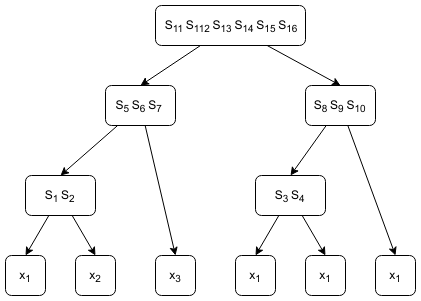
\includegraphics[width=0.5\textwidth]{Diagrames/totalizer.png}
    \caption{Representació Gràfica del arbre d'un totalizer}
    \label{fig:totalizer}
  \end{figure}

  Seguint amb l'exemple de la figura \ref{fig:totalizer} tindríem com a entrada el conjunt de variables $\{x_1, x_2, x_3, x_4, x_5, x_6\}$ i com a sortida el conjunt de variables $\{s_{11}, s_{12}, s_{13}, s_{14}, s_{15}, s_{16}\}$. És important notar que cada node codifica la cardinalitat de les fulles q en pengen, en format unari. Això significa que per tot i de cada node, $s_i \geq S_{i+1}$.

  En la figura \ref{fig:totalizer} també es poden veure totes les variables auxiliars que introdueix l'encoding per codificar un \textit{at-most-k} sobre 6 variables. Per veure quines clàusules genera, caldria definir un sumador unari, que donats dos nombres unaris, en retorni la suma en unari. 
  Aplicant-lo a cada node interior és suficient per garantir que $\{s_{11}, s_{12}, s_{13}, s_{14}, s_{15}, s_{16}\}$ és la representació unària de la cardinalitat de $\{x_1, x_2, x_3, x_4, x_5, x_6\}$. 
  Amb la representació unària de la cardinalitat, n'hi ha prou amb imposar que la interpretació de $out_{k+1}$ sigui falsa, per fer efectiu un, \textit{at-most-k}. 
 
  \paragraph*{Millores i optimitzacions} ~\\
  En la API SMT que s'ha utilitzat els encodings que s'han vist tenen aplicades certes millores per millorar la eficiència en clàusules i variables generades. A coninuació s'enumeren les millores:

  \begin{itemize}
    \item Sabem que \textit{at\_most\_one}, \textit{at\_least\_one} i \textit{exactly\_one} són
          un subconjunt de les restriccions de cardinalitat amb $k$, però amb $k=1$. Les codificacions d'aquestes (les quatre estudiades) són molt més eficients que quant no sabem la k, i, 
          per tant, és interessant tenir en compte que si $k=1$, en comptes d'utilitzar un \textit{sorter} o un \textit{totalizer}.
    \item Si en una restricció de cardinalitat diem que sobre un conjunt de $n$
          variables com a màxim $k$ han de ser certes (o sigui\textit{at\_most\_one(\{$v_1, ... ,v_n$\}, $k$ )})
          és el mateix que dir que com a mínim $n-k$ variables han de ser falses,
          (o sigui\textit{at\_least\_one(\{$\neg v_1, ... ,\neg v_n$\}, $n-k$ )}). Aquesta propietat també es pot aplicar de manera inversa. \\
          Quan $k$ és molt més gran que $n$, aquesta propietat ens pot ajudar a fer encodings molt més petits. 
          En la API SMT s'utilitza la següent relació: $k \geq n/2$.
    \item La codificació de un comparador binàri (molt utilitzat en els 2 encodings) es pot simplifcar en funció del operador utilitzat. En cas del exactament, necessitarem 6 clàusules. Pel $\leq$ 2, i pel $\geq$ només 1. Així es poden reduir les clàusules en les dues codificacions.
    \item Per últim, la API només codifica la circuiteria necessària per comparar fins a $k+1$, reduint molt la circuiteria necessària per a les diferents codificacions vistes.
  \end{itemize}




  \chapter{Requisits del sistema}

  En aquest treball es pretén desenvolupar un generador de horaris automàtic 
  amb SAT i/o SMT que serà capaç de rebre una instància XHSTT en un fitxer XML passat per paràmetre, 
  llegir-lo, codificar-ne un model utilitzant la API SMT desenvolupada pel Dr. Jordi Coll, resoldre'l i retornar un resultat, mostrant-lo per pantalla, o retornant un fitxer amb la instància XHSTT amb la nova solució inserida.

  Per fer-ho, serà necessari l'ús de un conjunt de llibreries i programari:

  \begin{itemize}
    \item Llibreria que permeti el tractament de fitxers XML, S'ha optat per pugixml\footnote{https://pugixml.org/}
    \item Posat que la API SMT utilitza Yices 2\footnote{https://yices.csl.sri.com/} com a únic \textit{solver} SMT, necessitarem tenir-ne la seva llibreria insta\l.lada.
    \item Posat que la API SMT està desenvolupada per GNU/Linux, serà necessari treballar una màquina que tingui insta\l.lat una distribució Linux.
  \end{itemize}
  
  Apart de tot el mencionat, també ha calgut decidir un país per el qual el generador d'horaris estarà desenvolupat. Això és degut a que en funció del país els requisits dels horaris generats varien àmpliament en funció de les característiques pròpies del sistema educatiu de cada país.
  En aquest treball s'ha decidit optar per les instàncies de Brazil, degut que tenen tots els recursos assignats a algun event, de manera que només es demana al generador organitzar els events, reduint l'espai de cerca.
 
 \begin{figure}[ht!]
  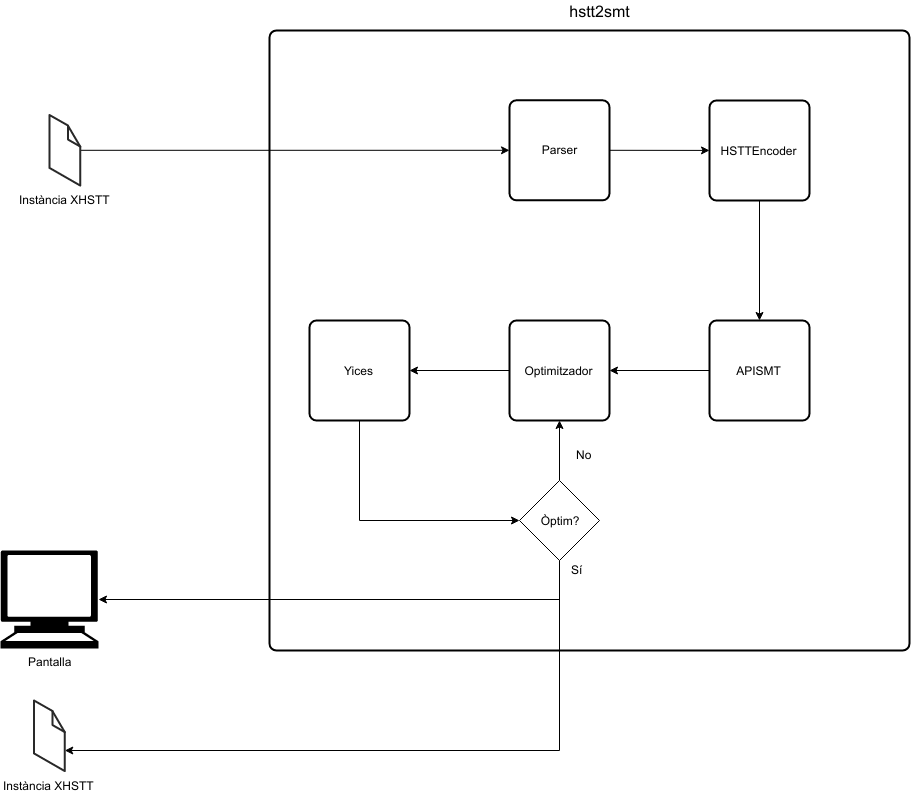
\includegraphics[width=\textwidth]{Diagrames/Arqui1.png}
  \caption{Arquitectura del programa}
  \label{fig:Arqui1}
\end{figure}
 

  \chapter{Estudis i decisions}
  \section{Programari utilitzat}
  En aquesta secció del treball es veurà tot el programari que s'ha utilitzat per la confecció d'aquest.
  \subsection{Yices 2}
  \begin{figure}[ht!]
    \centering
    
\includegraphics[width=0.4\textwidth]{Diagrames/logoYices.png}
    \caption{Logo Yices 2}
    \label{fig:yices}
  \end{figure}
  El Yices 2 és un \textit{SMT Solver} \textit{Open Source}\footnote{Repositori GitHub: \url{https://github.com/SRI-CSL/yices2}} sota llicència GPL que decideix la satisfactibilitat de fòrmules que contenen símbols de funcions no interpretades amb igualtat, aritmètica real i entera, BitVectors, tipus escalars i tuples. El Yices 2 suporta aritmètica linear i no linear.
  
  El Yices 2 pot processar fitxers d'entrada en notació SMT-LIB\footnote{\url{http://smtlib.cs.uiowa.edu/}}, es pot usar alternativament el llenguatge propi del Yices 2 i també te una API per C i C++.
  
  En la implementació d'aquest treball, s'usa dins de la API SMT del Dr. Jordi Coll com un dels \textit{solvers} que es poden utilitzar i és l'únic que permet SMT d'entre ells. S'ha decidit usar aquest a que és dels millors que hi ha i el grup de recerca hi te experiència prèvia. 

  S'ha utilitzat la versió 2.6.1.

  \subsection{pugixml}
  El pugixml és una llibreria C++ lleugera per al processament XML. És extremadament portable amb distribucions. També és opensource\footnote{Repositori GitHub: \url{https://github.com/zeux/pugixml}} sota llicència MIT.

  pugixml permet un processament de documents XML molt ràpid, còmode i eficient amb la memòria. Tot i això, al tenir un \textit{parser} DOM, no pot processar fitxers XML que no càpiguen a la memòria.
  
  Degut a les característiques mencionades i a experiència prèvia amb la llibreria, s'ha decidit utilitzar-la per a la programació del \textit{parser} XHSTT. 

  S'ha utilitzat en la versió 1.9-1.

  \subsection{C++}
  \begin{figure}[ht!]
    \centering
    
\includegraphics[width=0.2\textwidth]{Diagrames/cpp.png}
    \caption{Logo C++}
    \label{fig:cpp}
  \end{figure}
  
  Llenguatge de programació de propòsit general creat per Bjarne Stroustrup com a extensió del llenguatge de programació C. 
  Des de llavors, el llenguatge s'ha expandit molt i el C++ permet programació orientada a objectes, genèrica i funcional, a més de facilitats per manipulació de memòria a baix nivell. 
  Pràcticament sempre és implementat com a llenguatge compilat.

  El compilador per a C++ que s'ha utilitzat es el G++ inclòs en el GNU Compiler Collection, que inclou compiladors per a C, C++, Objective-C, Fortran, Ada, Go i D, a més de llibreries per aquests llenguatges. 
  

  \begin{figure}[ht!]
    \centering
    
\includegraphics[width=0.2\textwidth]{Diagrames/gcc.png}
    \caption{Logo G++}
    \label{fig:gpp}
  \end{figure}


  En aquest treball s'ha decidit utilitzar el C++ perquè és amb el que es treballa al grup de recerca i és amb el que està feta la API SMT. El C++ s'ha utilitzat en la revisió C++17 del seu estàndard. El GCC utilitzat ha estat en la versió 9.1.0-2. 

  % \subsection{QtCreator}

  % \begin{figure}[ht!]
  %   \centering
  %   
\includegraphics[width=0.2\textwidth]{Diagrames/qtc.png}
  %   \caption{Logo QtCreator}
  %   \label{fig:qtc}
  % \end{figure}

  % El QtCreator és un Entorn de Desoenvolupament Integrat (IDE de \textit{Integrated Development Environment}) multiplataforma per a C++, 
  % JavaScript i QML que forma part del SDK per el \textit{framework} de desenvolupament d'aplicacions amb GUi Qt. Utilitza 

  % S'ha utilitzat la versió 4.9.2-3.

  \subsection{\LaTeX}
  \begin{figure}[ht!]
    \centering
    
\includegraphics[width=0.4\textwidth]{Diagrames/latex.png}
    \caption{Logo \LaTeX}
    \label{fig:latex}
  \end{figure}
  

  Aquesta memòria s'ha confeccionat amb \LaTeX, que és un sistema de composició d'alta qualitat que inclou funcions dissenyades per a la creació de documents tècnics i científics amb la intenció de ajudar al creador a centrar-se més en el contingut que en la forma.
\LaTeX és l'estàndard de facto per a la comunicació i publicació de documents científics. 

Per la confecció i edició del document en sí, s'ha utilitzat l'editor Open Source\footnote{Link GitHub: \url{https://github.com/Microsoft/vscode}} Visual Studio Code. S'ha utilitzat en la versió 1.37.1-2 amb extensions per a facilitar l'edició del document tex.



  \subsection{GNU/Linux}
  \begin{figure}[ht!]
    \centering
    
\includegraphics[width=0.2\textwidth]{Diagrames/Linux.png}
    \caption{Logo Linux}
    \label{fig:linux}
  \end{figure}
  Linux és una família de sistemes operatius formats pel \textit{kernel} Linux juntament amb les utilitats GNU. 
  El generador que s'ha fet en aquest treball ha estat desenvolupat per a Linux, degut a la facilitat d'accés a les múltiples llibreries que s'han utilitzat, a que la API SMT ha estat desenvolupada també per a Linux i simplement per preferència personal, degut a que el sistema operatiu que utilitzo dia a dia és una distribució Linux.

  En concret s'ha treballat amb la distribució Arch Linux en la versió del kernel Linux 5.29.arch1-1 al final del treball (s'han usat versions anteriors que han anat sortint mentre es desenvolupava el treball).


  \section{Maquinari utilitzat}
  Per efectuar les proves de rendiment s'ha utilitzat un ordinador amb les següents especificacions:
  \begin{itemize}
    \item Processador AMD Ryzen\textsuperscript{TM} 3 1200 a 3.5 GHz amb 4 nuclis físics,  10MB de memòria cau i arquitectura 64 bits.
    \item 16GB de memòria RAM DDR4 a 3333MT.
    \item Sistema operatiu Arch Linux 64 bits amb kernel Linux 5.2.9.arch1-1
  \end{itemize} 
  


  \chapter{Anàlisis i disseny del sistema}

  En aquest capítol s'estudien les diferents necessitats del generador d'horaris automàtic que es pretén desenvolupar al llarg del treball
  i es planteja com solucionar-les. 
  Es presenten propostes de com funcionarà internament l'aplicació, 
  com es guardaran les diferents dades que necessitem i com es comunicarà amb l'usuari. 



  \section{Anàlisis}
  % En la fase d’anàlisi cal detallar el model de dades i el model de processos. 
  \subsection{Necessitats del sistema}
  Les necessitats principals del sistema són les següents: 
  \begin{itemize}
    \item Necessitem rebre un fitxer de l'usuari.
    \item Necessitem llegir les dades de un fitxer XHSTT tal i com s'ha explicat anteriorment, per tant requerirem de un \textit{parser} per fer-ho.
    \item Necessitarem guardar les dades i les restriccions de alguna manera.
    \item Necessitarem un model lògic i codificar-lo utilitzant la API SMT del Dr. Jordi Coll. 
    \item Necessitarem processar i guardar les dades de manera que ens faciliti el mostrar-les de forma que es pugui entendre.
    \item Necessitarem comprovar en la mesura del possible que la instància XHSTT sigui correcta.
  \end{itemize}

  \subsection{Anàlisis de processos}
  L'usuari cridarà el programa, el programa llegirà el fitxer XHSTT que li ha passat l'usuari per paràmetre i s'encarregarà de codificar el model pel yices i cridar-lo per resoldre'l, utilitzant la llibreria per C++ pròpia del Yices 2.
  %AMPLIAR + dibuixet un dibuixet amb lo de requeriments mes enfocat als processos
  \begin{figure}[p]
    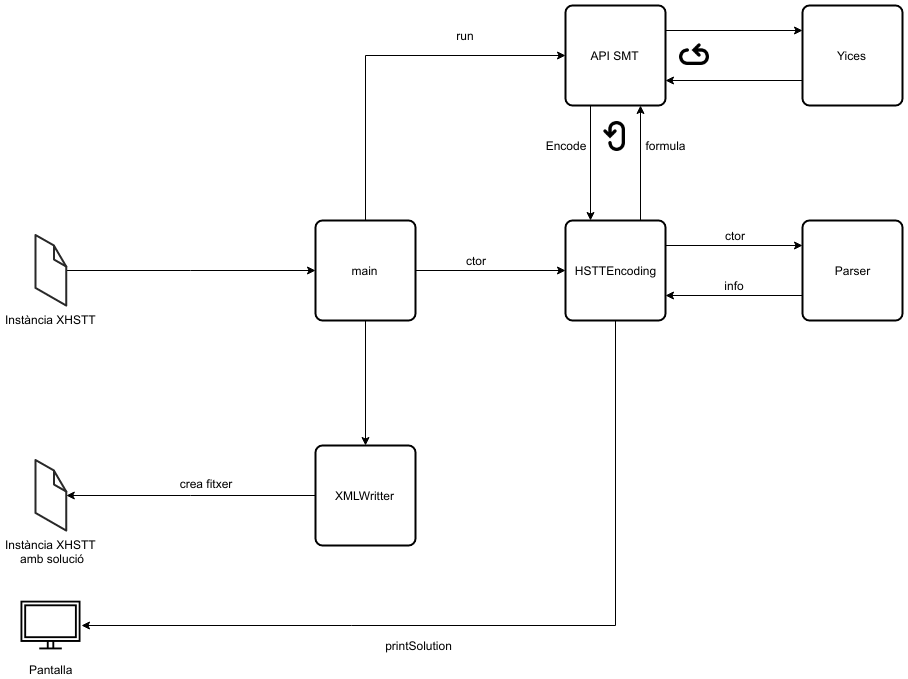
\includegraphics[width=\textwidth]{Diagrames/Arqui2.png}
    \caption{Esquema de processos}
    \label{fig:procs}
  \end{figure}
  

  
  \section{Disseny}    
  % En la fase de disseny cal determinar les interfícies d’usuaris, els models físics de 
  % dades, (no cal)els models físics de processos i, si escau, el model d’objectes. En aquest 
  % àmbit, els patrons de disseny permeten reutilitzar solucions generals a problemes 
  \subsection{Interfícies d'usuari}
  El programa funcionarà via consola. Les dades necessàries, com ara el fitxer amb la instància, es passaran per paràmetres, utilitzant el sistema existent en la API SMT del Dr. Jordi Coll.
  \subsection{Model de dades}

  El model de dades correspondria al següent diagrama:
  \begin{figure}[H]
    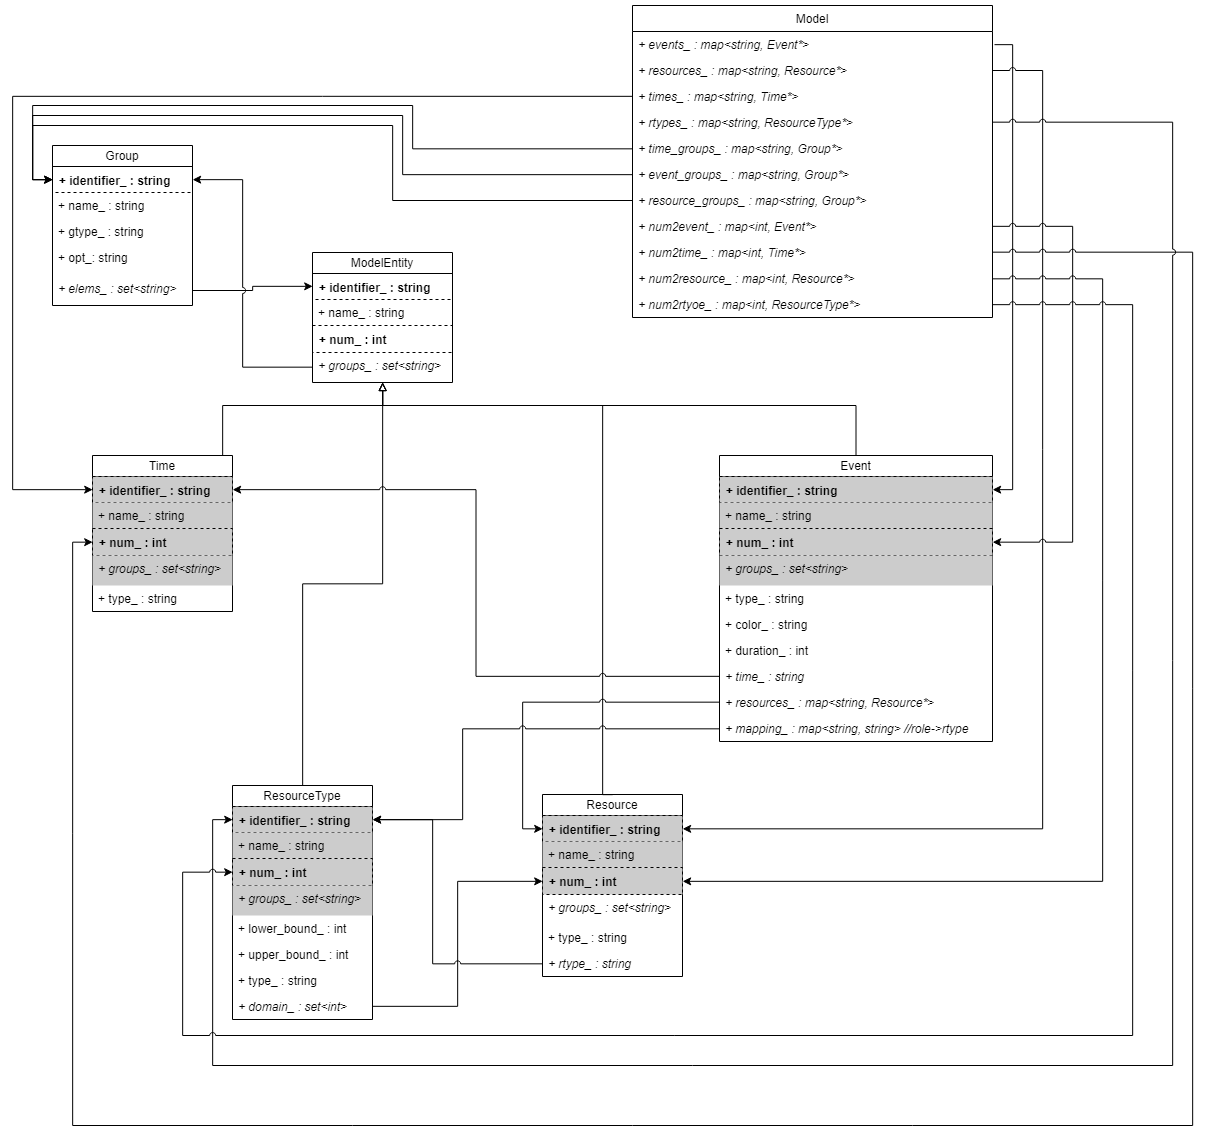
\includegraphics[width=\textwidth]{Diagrames/ModelDades.png}
    \caption{Model de Dades}
    \label{fig:DataModel}
  \end{figure}

  Com es pot veure en la figura \ref{fig:DataModel}, la classe \textit{Model} guarda la informació de la instància (sense incloure les restriccions). D'aquesta heretaran tots els encodings que es puguin arribar a fer, posat que sempre serà el mateix.
  Per fer-ho s'ha creat la classe \textit{ModelEntity} de la qual hereten les classes \textit{Event}, \textit{Resource}, \textit{ResourceType} i \textit{Time},
  representant respectivament a les assignatures, els recursos, els tipus de recursos i els espais de temps disponibles. Aquestes classes mantenen tota la informació necessària per a representar a cada tipus d'element. La classe \textit{ModelEntity}
  inclou un identificador  únic de tipus \textit{string} i un numero enter unic per cada un dels tipus existents. Hi poden haver un \textit{Event} i un \textit{Resource} amb el mateix número, però mai hi haurà dos elements del mateix tipus amb el mateix numero.

  A més s'ha creat una classe \textit{Group} per tal de mantenir els diferents grups d'elements d'elements que preveu XHSTT.  


  \subsection{Model d'objectes}

  El model d'objectes correspondria al següent diagrama:
  \begin{figure}[H]
    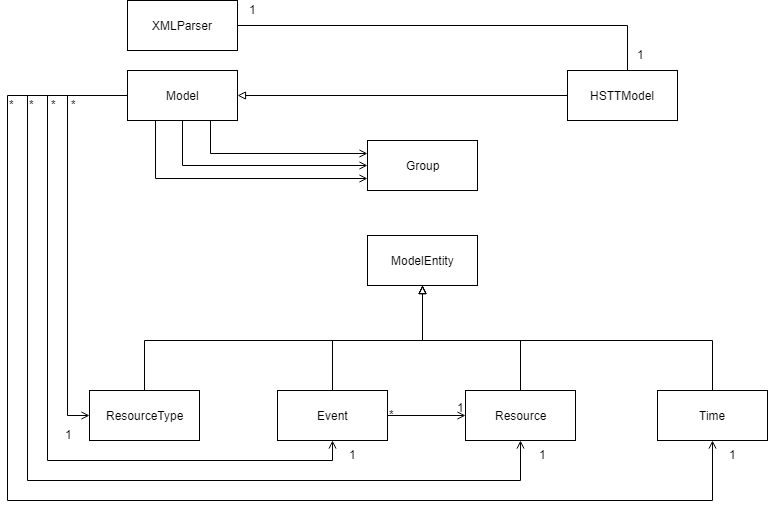
\includegraphics[width=\textwidth]{Diagrames/UMLKai.png}
    \caption{Model d'objectes}
    \label{fig:ObjectModel}
  \end{figure}
  

  El programa consistirà en un objecte HSTTEncoding al qual donarem el nom del fitxer que volem llegir i treballarà amb ell. 
  El HSTTEncoding crearà l'objecte XMLParser per tal de llegir el fitxer i es comunicaran entre ells mentre XMLParser vagi llegint el fitxer enviant la informació llegida al HSTTEncoding. 
  Al heretar de Model, aquest pot guardar totes les dades, que consistiran en diferents tipus de \textit{ModelEntity} i diferents \textit{Groups}.
  Des de aquí HSTTEncoding s'encarregarà de resoldre la instància comunicant-se amb la API SMT.

  \subsection{API SMT}

  La API SMT desenvolupada pel Dr. Jordi Coll serà molt utilitzada durant el desenvolupament del treball.
  Aquesta API ens fa d'interfície per a codificar de forma senzilla i intuïtiva 
  problemes de satisfacció de restriccions utilitzant SAT, MaxSAT o SMT. 
  Això ens ho permet fer de manera independent del solver i, fins i tot,
  ens permet extreure la codificació del problema que s'estigui treballant 
  en fitxers de format \textit{SMT-LIB}\footnote{\url{http://smtlib.cs.uiowa.edu/language.shtml}} o 
  \textit{dimacs} \footnote{\url{https://people.sc.fsu.edu/~jburkardt/data/cnf/cnf.html}}.

  Aquesta API, a més del mencionat, 
  té codificades les diferents restriccions de cardinalitat mencionades en la secció \ref{card}. Això ens permetrà centrar-nos en implementar el model sense haver-nos de preocupar de codificar les diferents restriccions de cardinalitat vistes.



  

  \chapter{Implementació i proves}

  La implementació del generador s'he fet en C++, i està format per un conjunt de blocs definits:\
  \begin{itemize}
    \item \textit{Parser }del fitxer en format XHSTT. \\ S'encarrega de llegir el fitxer XHSTT i extreure'n la informació de la instància continguda en el fitxer XML en format XHSTT passat per paràmetre. És important que aquest fitxer tingui l'estructura establerta en el format XHSTT.
    \item Bloc de codificació de la instància a SMT. \\ En aquest apartat utilitzem la API SMT per tal de codificar la instància a SMT i passar-la al \textit{solver} corresponent, el Yices 2.
    \item Bloc de escriptura del resultat a XHSTT. \\ En aquest apartat creem un fitxer amb la instància treballada XHSTT i hi afegim la solució trobada al final.
  \end{itemize}

  L'usuari només tindrà un binari, anomenat \textit{hstt2smt}, amb el qual interactuarà per resoldre una instància que passarà per fitxer. Aquest s'encarregarà de fer tota la feina i mostrarà per pantalla el resultat, a part també creara un fitxer en la carpeta \textit{output} amb la instància treballada, afegint-hi la solució trobada en el format XHSTT
  Aquest binari serà el resultat de compilar el generador amb la API SMT i les llibreries que es necessiten per poder treballar amb XML i amb SMT.
  %%%REVISAR%%%%%

  \section{Parser XHSTT}

  El parser XHSTT consisteix en una classe que llegeix una instància XHSTT i passa la informació al model per que aquest pugui fer la codificació de les diferents restriccions.

  El funcionament del parser segueix el següent esquema:

  \begin{enumerate}
    \item Llegir element de la instància (Event, espai de temps o recurs) i enviar les dades al Model que se les guardarà.
    \item Al acabar de llegir els elements, enviar una senyal al codificador per a què faci les variables del model i les restriccions de \textit{channeling}.
    \item Llegir restricció i enviar les dades a \textit{HSTTEncoding} per a què les codifiqui.
  \end{enumerate}

  \section{Codificació}
  En aquesta secció es descriu la implementació de la codificació a SMT del generador d'horaris. 
  Posat que SMT no permet clàusules violables, per a la codificació d'aquesta s'utilitzarà el cost i una variable auxiliar per cada clàusula \textit{soft}, 
  que s'afegira a la seva corresponent clàusula de forma condicional, negant la clàusula inicial, de manera que si no es compleix la clàusula inicial, la variable auxiliar hagi de ser certa. Al acabar la codificació de la instància afegirem una clàusula pseudo-booleana amb totes les variables auxiliars amb els seus pesos, comparada amb un upperbound.
  Posat que la funció d'optimització serà la de minimitzar el cost total, el optimitzador anirà modificant el upperbound intentant reduir la funció objectiu, que també és el resultat exacte de la pseudo-booleana.

  Per exemple, si tenim les \textit{soft-clauses} següents: $SC_1$, $SC_2$, $SC_3$ amb costos respectivament: $W_1$, $W_2$, $W_3$. 
  Crearíem les variables auxiliars $Aux_1$, $Aux_2$ i $Aux_3$. Amb això crearíem les següents clàusules:
  \begin{gather*}
    \neg SC_1 \rightarrow Aux_1 \\
    \neg SC_2 \rightarrow Aux_2 \\
    \neg SC_3 \rightarrow Aux_3
  \end{gather*}

  Hi aplicaríem Àlgebra de Bool per convertir a CNF i convertiríem les clàusules que són tipus $\neg A \rightarrow B$ a $\neg (\neg A) \vee B$ i d'aquí eliminaríem la doble negació, quedant $A \vee B$:
  \begin{gather*}
    \neg SC_1 \vee Aux_1 \\
    \neg SC_2 \vee Aux_2 \\
    \neg SC_3 \vee Aux_3
  \end{gather*}
  Així doncs, afegint la clàusula pseudo-booleana amb les variables auxiliars i els pesos, ens quedarien les següents clàusules:
  \begin{gather*}
      SC_1 \vee Aux_1 \\
      SC_2 \vee Aux_2 \\
      SC_3 \vee Aux_3 \\
      Aux_1*W_1 + Aux_2*W_2 + Aux_3*W_3 <= UPPERBOUND
  \end{gather*}


  Aquesta codificació està pensada per resoldre instàncies en què tots els recursos estan assignats a algun event, com ara les instàncies de Brazil que són en les que ens hem enfocat al desenvolupar el generador. 
  Aquesta particularitat ens permet simplificar l'espai de cerca degut a la reducció de la combinatòria del problema, i permet una codificació més simple i directe de les restriccions de que es compon.

  \subsection{Model}

  El model està pensat per treballar a centrant-nos en els Events, els quals podríem definir com una reunió a la que es presenten diferents recursos i la nostre feina és la de decidir en quins espais de temps dels disponibles fiquem cada reunió d'aquestes.

  Les variables del model són les següents:
  \begin{itemize}
    \item $Xt_{0,0} . . . Xt_{|Events|-1,|Times|-1}$\\Per cada event tenim tantes variables com espais de temps tingui la instancià. Cada una d'aquestes variables indica si un event en un espai de temps, s'està celebrant o no. 
    Doncs si per l'event $e$ i l'espai $t$, $Xt_{e,t}$ és certa, vol dir que en el temps $t$, $e$ s'està celebrant.
    \item $Xs_{0,0} . . . Xs_{|Events|-1,|Times|-1}$\\Per cada event tenim tantes variables com espais de temps tingui la instància. Cada una de aquestes variables indica si un event comença en l'espai de temps representat. Un event comença en un espai de temps si no es donava en l'espai de temps anterior i/o si l'espai de temps és la primera hora del dia.
    Doncs si per l'event $e$ i l'espai $t$, $Xt_{e,t}$ és certa, vol dir que en el temps $t$, $e$ comença i que cap més variable $Xs_{e,i}$ serà certa i que la variable $Xt_{e,t}$ serà certa.
    \item $Xd_{0,1,0} . . . Xd_{|Events|-1, event.duration, |Times|-1}$\\ Per cada event i cada possible duració d'aquest tenim una variable. Per exemple, si per a un event de duració 5, es defineixen fins a 5 conjunts de $|Times|$ variables. 
    Cada variable ens indica si comença una lliçó de la durada i en l'espai de temps que representa la variable. 
  \end{itemize}

  \subsection{Clàusules de Channeling}

  Per poder dotar les variables del model de semàntica caldrà afegir certes clàusules. A continuació s'enumeren:
  \begin{itemize}
    \item Si un event comença a una hora determinada, llavors té una duració: \begin{center} $\forall e \in 0 ... |Events|-1$ $\forall i \in 0 ... |Times|-1$ \\$exactily\_one(\neg Xs_{e,i} \vee \{ \forall j \in 1 ... e.duration$ $Xd_{e,j,i}\})$\end{center}
    \item Si un event té lloc a t però no a t-1, és que comença: \begin{center} $\forall e \in 0 ... |Events|-1$ $\forall i \in 0 ... |Times|-1$ \\$\neg Xt_{e,i} \vee Xt_{i-1} \vee Xs_i$ \end{center}
    \item Si un event comença amb duració d, llavors té lloc en d hores consecutives: \begin{center} 
      $\forall e \in 0 ... |Events|-1$ $\forall d in 1 ... e.duration$ $\forall i \in 0 ... |Times|-1$ $\forall j \in i ... i+d-1$ \\
      $\neg Xd_{e,d,i} \vee Xt_{e,j}$
    
    \end{center}
  \end{itemize}

  \subsection{Restriccions XHSTT}
  \paragraph*{Assign Times Constraint} ~\\~\\
  
  Restricció per imposar que a tots els events se'ls hi assigni temps. Per tant, per a cada event $e$ hem de imposar que del conjunt de variables $Xt{e,i}$, n'hi hagi exactament $e.duration$ que s'avaluïn a Cert:
  \[
    \forall e \in Events \ exactly_k(\{Xt_{e,0} ... Xt_{e,|Times|-1}\}, e.duration)
  \]

  \paragraph*{Split Events Constraint} ~\\~\\ 
  Aquesta restricció limita la manera en com es fragmenten els events. És a dir, sobre el nombre de sessions en què es fragmenta i la durada d'aquestes.\\
  Per a la restricció sobre el nombre de sessions en què es fragmenta un event, utilitzarem les tags de \textit{MinimumAmount} i \textit{MaximumAmount} per fer les següents clàusules:
  \begin{gather*}
    \forall e \in Events \ at\_most\_k(\{Xs_{e,0} . . . Xs_{e,|Times|-1}\}, MaximumAmount)\\
    \forall e \in Events \ at\_least\_k(\{Xs_{e,0} . . . Xs_{e,|Times|-1}\}, MinimumAmount)
  \end{gather*}

  Pel que fa el control de la durada de les sessions nomes cal negar totes les variables Xd de cada event que corresponguin a duracions q no estiguin compreses entre el rang definit per les tags \textit{MinimumDuration} i \textit{MaximumDuration}:
  \begin{gather*}
    \forall e \in Events \ \forall d \notin MinimumDuration...MaximumDuration \land d \in 1 ... e.duration  \\
    \forall t \in 0...|Times|-1 \quad \neg Xd_{e,d,t}
  \end{gather*}

  \paragraph*{Distribute Split Constraint} ~\\~\\

  Restricció que limita el nombre de events d'una duració determinada, per tant limita la cardinalitat de variables $Xd$. $d$ ve donada per la tag \textit{Duration} i el màxim i mínim venen donats per les tags \textit{Maximum} i \textit{Minimum}:
  \begin{gather*}
  \forall e \in Events \ at\_most\_k(\{Xd_{e,d,0} .... Xd_{e,d,|Times|-1}\}, max) \quad \quad si \ max<\frac{e.duration}{d}\\
  \forall e \in Events \ at\_most_k(\{Xd_{e,d,0} .... Xd_{e,d,|Times|-1}\}, min) \quad \quad \quad si \ min>0\\
  \end{gather*}


  \paragraph*{Prefer Times Constraint} ~\\~\\
  
  Restricció que indica en quins espais de temps no es poden programar certes sessions. Per exemple, pot servir per indicar que no es pot programar una sessió de dues hores en la última hora del dia.

  Definim el conjunt $Ta$ com el conjunt de slots de temps els quals la restricció ens diu que són preferits. Neguem totes les variables $Xd$ de duració d que representin espais de temps no continguts dins de Ta.
  \begin{gather*}
    \forall e \in Events \ \forall t \in Times \land t \notin Ta \\ (\neg Xd_{e,d,t})
  \end{gather*}


  \paragraph*{Spread Events Constraint} ~\\~\\
  
  Aquesta restricció posa límits en el nombre de sessions de cada event que es poden celebrar en certs grups d'espais de temps definits com a dies.

  Definim $Tg$ com el conjunt grups d'espais de temps definits per la restricció.

    \begin{align*}
      \forall e \in Events \ &\forall g \in Tg \\
      &at\_most\_k(\{Xs_{e,t} | t \leftarrow g\}, max)\\
      \forall e \in Events \ &\forall g \in Tg \\
      &at\_least\_k(\{Xs_{e,t} | t \leftarrow g\}, max)
    \end{align*}


  \paragraph*{Avoid Clashes Constraint} ~\\~\\

    Aquesta restricció imposa que certs recursos no poden tenir assignats més d'un event al mateix temps. 
    Aquí aprofitem que els recursos estan assignats d'un inici, i definim $E_r$ com el conjunt de events als quals ha de assistir un recurs $r$ i imposem que per cada espai de temps, com a molt un d'els events de E pot estar programat:
    \begin{align*}
      \forall r \in Resources \ & \forall t \in Times \\
      &at\_most\_one(\{Xt_{e,t} | e \leftarrow E_r\})
    \end{align*}

  \paragraph*{Avoid Unavailable Times Constraint} ~\\~\\

  Restricció que indica que hi ha certs espais de temps durant les quals no podem utilitzar certs recursos. $T$ és conjunt d'espais de temps no disponibles i $E_r$ el conjunt d'events als que ha d'assistir un recurs $r$:
  \begin{align*}
    \forall r \in Resources \ \forall t \in T \ \forall e \in E_r \quad
    (\neg Xt_{e,t})
  \end{align*}
    
    
  \paragraph*{Limit Idle Times Constraint} ~\\~\\

  Restricció que limita el nombre d'espais de temps lliure entre dos espais de temps ocupats a l'horari de certs recursos. 
  Per tal de codificar aquesta restricció és necessari afegir variables auxiliars al model. Per cada espai de temps que pot ser forat s'introdueix una variable auxiliar que serà certa si l'espai realment és un forat.

  El conjunt $Tg$ representa el conjunt de grups d'espais de temps que tractem. 
  S'introdueix la variable $idle_i$ per cada recurs que defineix si aquest té un forat en l'horari en l'espai de temps $i$. Per tal de considerar un espai de temps com a forat, cal que en algun moment abans i després hi hagi programada alguna activitat.
   Així que es defineixen dos conjunts: $A_i$ representant els espais de temps posterior (\textit{After}) de $i$ i $B_i$ representant els espais de temps anteriors (\textit{Before}) de $i$.
   
   Llavors, per a cada recurs $r$ es fan les següents clàusules:
   \begin{align*}
    \forall g \in Tg \ \forall t \in g \ &\forall e \in E_r \\
    &(\neg Idle_i \lor \neg Xt_{e, t}) & si \ \ (B_t \neq \emptyset \ \& A_t \neq \emptyset) \\
    \forall g \in Tg \ \forall t \in g  \ & \\
    & (\neg Idle_t \lor \{\forall b \in B_t \ \forall e \in E_r \ Xt_{e,b}\}) & si \ \ (B_t \neq \emptyset)\\
    \forall g \in Tg \ \forall t \in g & \\
    & (\neg Idle_t \lor \{\forall a \in A_t \ \forall e \in E_r \ Xt_{e,a}\}) & si \ \ (A_t \neq \emptyset)\\
    \forall g \in Tg \ \forall t \in g \ \forall b \in B_t \ \forall a \in A_t & \\
    \forall e1 \in E_r \ \forall e_2 \in E_r \ \forall e_3 \in E_r & \\
    & (Xt_{e_{1}, t} \lor \neg Xt_{e_2, b} \lor Xt_{e_3, a} \lor Idle_t) & si \ \ (B_t \neq \emptyset \ \& A_t \neq \emptyset)
   \end{align*}

   Un cop definides i lliguades les variables auxiliars l'únic que queda és, per cada recurs, imposar les restriccions de cardinalitat:

   \begin{align*}
    \forall r \in Resources &\\
    & at\_most\_k(\{ Idle_t | t \leftarrow Times\}, max) \\
    & at\_least\_k(\{ Idle_t | t \leftarrow Times\}, min)
   \end{align*}

  \paragraph*{Cluster Busy Times Constraint} ~\\~\\

  Restricció que imposa límits sobre el nombre de grups d'espais de temps (que podem entendre com a dies) en què un recurs pot estar ocupat. En aquesta restricció introduirem una variable $Busy_g$ per a cada recurs que ens indicarà si el recurs està ocupat en el grup $g$ o no.

  Per a cada recurs $r$ es fan les clàusules següents:
  
  \begin{align*}
    \forall g \in Tg & \\
    &(\neg Busy_g \lor (\forall e \in E_r \ \forall t \in g \quad Xt_{e,t}))\\
    \forall g \in Tg \ \forall t \in g \ \forall e \in E_r &\\
    & (\neg Xt_{e,t} \lor Bsuy_g)
  \end{align*}

  Un cop definides i lligades les variables auxiliars l'únic que queda és, per cada recurs, imposar les restriccions de cardinalitat:
  \begin{align*}
    \forall r \in Resources &\\
    & at\_most\_k(\{ Busy_g | g \leftarrow Tg\}, max) \\
    & at\_least\_k(\{ Busy_g | g \leftarrow Tg\}, min)
   \end{align*}
  


   \section{Proves}

   Les proves del programa desenvolupat s'han dividit en dos fases: el parser i el generador automàtic d'horaris sencer. 
   Això s'ha fet així per assegurar que quan es comences a dissenyar el model, les dades rebudes per aquest fossin sempre correctes. Així doncs, abans de començar a fer la codificació en sí, s'ha fet i provat el parser.

   Per fer les proves tant del parser com del programa sencer s'ha utilitzat el mètode de la caixa negra\cite{wiki:blackbox}. Aquest mètode consisteix en examinar el funcionament del programari que està sent provat sense tenir en compte el com està implementat, com un tot. 
   La idea està en provar els casos d'ús de forma independent al codi intern en sí i comparar els resultats amb els que s'esperaven.
   
   Aquest mètode busca trobar errors en:
    \begin{itemize}
      \item Funcions incorrectes o inexistents
      \item Errors de interfície
      \item Errors en les estructures de dades
      \item Errors en el comportament o en el rendiment
      \item Errors de inicialització i terminació
    \end{itemize}


  % En aquest apartat es detallen els problemes i les solucions apareguts en la 
  % implementació, així com, si és el cas, el model de classes i els algorismes més 
  % rellevants. 
  
  % A més, cal detallar les proves, tant unitàries com de sistema, que es realitzen. 
    
  \chapter{Resultats}
  % Aquest apartat ha de descriure amb detall el procés de desenvolupament que ha 
  % calgut dur a terme per implantar el sistema desenvolupat. L’apartat de resultats ha 
  % de mostrar clarament el grau d’assoliment dels objectius, mitjançant exemples del 
  % funcionament d’allò que s’ha fet. 
   
  % Es revisarà i valorarà que el sistema desenvolupat compleixi amb la legislació i 
  % normatives vigents, especialment en el que fa referència a la llei orgànica de 
  % protecció de dades de caràcter personal (LOPD) i a la llei de serveis de la societat 
  % de la informació i comerç electrònic (LSSICE). 
   
  % A més, ha de mostrar que l’aplicació resultant del projecte fa les tasques 

  En aquesta secció es realitzarà una comparativa de rendiment amb els diferents encodings diferents en la API SMT i es veuran els resultats donats per el generador per les diferents instàncies de Brazil que es poden trobar en el repositori públic.

  El format XHSTT disposa d'un avaluador d'horaris online anomenat HSeval\cite{hseval}. Aquest, ens serveix per avaluar la bondat d'un horari i, a més, permet mostrar-lo de forma gràfica. 
  Aquesta eina ens permetrà comprovar com de bona és cada solució comparada amb les ja existents.
  A continuació es mostraran els resultats obtinguts amb la instància \textit{BrazilInstance1.xml} en la web i en el generador en sí, que també mostra els horaris resultants per pantalla, com es pot veure a la figura \ref{fig:bi1_term}. 

  Per aconseguir l'informe de resultats només cal pujar el fitxer xml amb la solució, seleccionar la opció \textit{HTML Report} i fer click a \textit{Submit}. El resultat es pot veure a la figura \ref{fig:bi1_report}.
  Per aconseguir la representació gràfica dels horaris, en comptes de seleccionar \textit{HTML Report}, triem la opció \textit{HTML Timetables}. 
  Aquesta opció generarà un horari per cada Recurs (en les instàncies de Brazil serien un per cada professor, com veiem a la figura \ref{fig:bi1_teach}, i un per cada classe, com es pot veure en la figura \ref{fig:bi1_class}). 

  Els resultats mostrats a continuació, són els obtinguts de optimitzar la \textit{BrazilInstance1.xml}. \newpage

  \begin{figure}
    \centering
    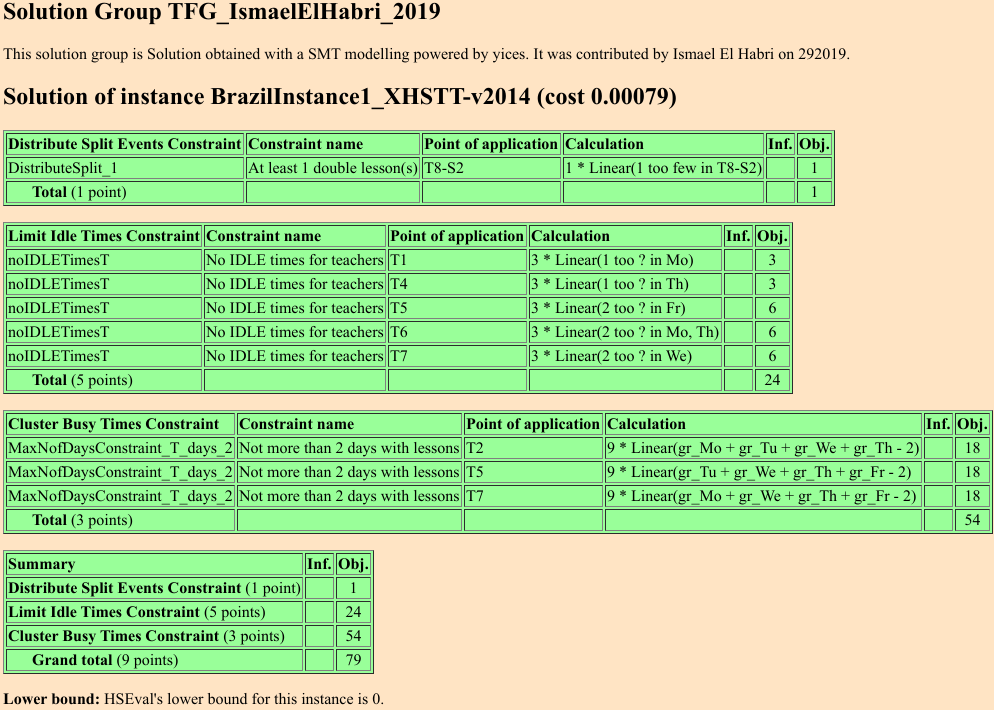
\includegraphics[width=\textwidth]{Diagrames/brazil1_report.png}
    \caption{Informe d'optimalitat obtingut amb HSEval}
    \label{fig:bi1_report}
  \end{figure}
  \newpage
  \begin{figure}[H]
    \centering
    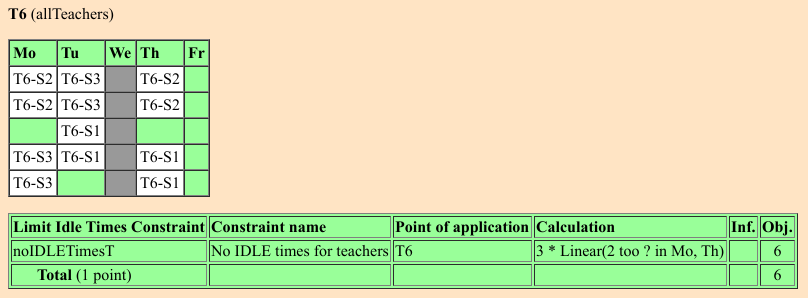
\includegraphics[width=\textwidth]{Diagrames/brazil1_teach.png}
    \caption{Horari d'un professor de \textit{BrazilInstance1.xml}}
    \label{fig:bi1_teach}
  \end{figure}
  % \begin{figure}
  %   \centering
  %   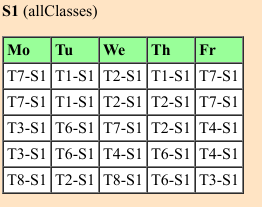
\includegraphics[width=0.8\textwidth]{Diagrames/brazil1_class.png}
  %   \caption{Horari d'unes classes de \textit{BrazilInstance1.xml}}
  %   \label{fig:bi1_class}
  % \end{figure}
  \begin{figure}[H]
    \centering
    \begin{subfigure}[b]{0.45\linewidth}
      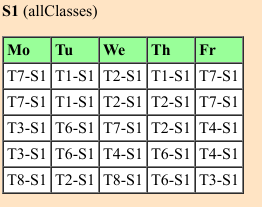
\includegraphics[width=\linewidth]{Diagrames/brazil1_class.png}
    \end{subfigure}
    \begin{subfigure}[b]{0.45\linewidth}
      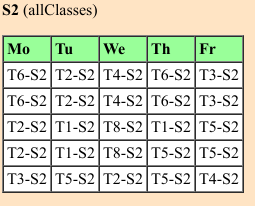
\includegraphics[width=\linewidth]{Diagrames/brazil1_class2.png}
    \end{subfigure}
    \caption{Horari d'unes classes de \textit{BrazilInstance1.xml}}
    \label{fig:bi1_class}
  \end{figure}
  \begin{figure}[htp!]
    \centering
    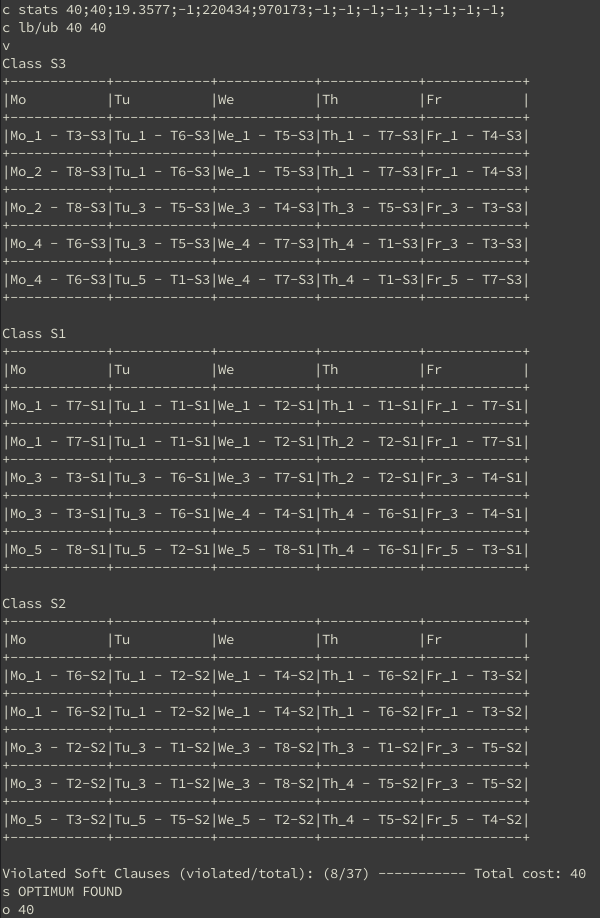
\includegraphics[width=0.8\textwidth]{Diagrames/brazil1_terminal.png}
    \caption{Resultat de la instància 1 des de el generador d'horaris.}
    \label{fig:bi1_term}
  \end{figure}
  \newpage

  \section{Comparativa d'encodings}

  En aquest apartat es provaran tots els encodings de les clàusules de cardinalitat (bàsicament \textit{at\_most\_one} i \textit{at\_most\_k}) disponibles en la API SMT i es mirarà com afecten aquests en el rendiment del generador d'horaris. 
  Totes les proves realitzades en aquesta secció seran de resolució. En totes les proves d'execució s'ha utilitzat un temps límit de 30 minuts.

  \subsection{Comparativa per temps d'execució}

  \paragraph*{Encoding Cardinalitat: Sorter} ~\\

  Aquí es presenta una taula amb els temps d'execució amb els diferents encodings disponibles del \textit{at\_most\_one} combinats amb el encoding de cardinalitat \textit{sorter}:
  \begin{figure}[ht!]
    \centering
    \begin{tabular} { c | c c c}
      Encoding & BrazilInstance1 & BrazilInstance2 & BrazilInstance3 \\
      \hline
      Quadràtic &   1.052 & 6.450 & 10.331 \\
      Logarítmic &  1.126 & 6.151 & 10.989 \\
      Ladder &      1.275 & 6.084 & 12.492  \\
      Heule &       1.242 & 6.437 & 11.815  \\
    \end{tabular}
    \caption{Taula de resultats de temps de les instàncies de la 1 a la 3}
    \label{fig:taula1}
  \end{figure}

  \begin{figure}[ht!]
    \centering
    \begin{tabular} { c | c c c c}
      Encoding & BrazilInstance4 & BrazilInstance5 & BrazilInstance6 & BrazilInstance7 \\
      \hline
      Quadràtic &   02:56.91 & 28.63 &  35.45 & 01:52.45 \\
      Logarítmic &  11:38.62 & 28.753 & 39.163 & 01:48.02 \\
      Ladder &      Timeout &  31.018 & 39.797 & 02:22.87 \\
      Heule &       05:03.38 & 28.934 & 40.441 & 02:38.68 \\
    \end{tabular}
    \caption{Taula de resultats de temps de les instàncies de la 4 a la 7}
    \label{fig:taula2}
  \end{figure}

  Al veure els resultats el primer que salta a la vista és el fet de que la instància 4 sigui la més lenta en resoldre's, sent els seus temps d'execució molt diversos i amb una diferència de temps entre encodings molt gran. En el millor dels casos 
  tarda menys de 3 minuts en resoldre's, aquest és amb la codificació quadràtica. Les codificacions logarítmica i Ladder són molt pitjors en temps d'execució que la resta en aquesta instància, tardant la primera més de 10 minuts i la segona fent saltar el límit de temps de 30 minuts.

  En general es pot observar que la instància quadràtica ofereix uns resultats en temps d'execució molt competitius, sent la millor en totes les instàncies de la taula corresponent a la figura \ref{fig:taula2} 
  menys la setena, on la millor codificació és la logarítmica per aproximadament 4 segons.
  Pel que fa a les corresponents a la figura \ref{fig:taula1}
  el quadràtic aconsegueix també el millor temps en totes menys la segona instància, pero sent les diferències de temps tant petites en aquestes instàncies, es podria simplement considerar marge d'error. 

  Pel que fa la resta de codificacions es pot veure que, en funció de la instància unes tenen millor rendiment que d'altres.

  \paragraph*{Encoding Cardinalitat: Totalizer} ~\\

  Aquí es presenta una taula amb els temps d'execució amb els diferents encodings disponibles del \textit{at\_most\_one} combinats amb el encoding de cardinalitat \textit{totalizer}:
  \begin{figure}[ht!]
    \centering
    \begin{tabular} { c | c c c}
      Encoding & BrazilInstance1 & BrazilInstance2 & BrazilInstance3 \\
      \hline
      Quadràtic &  1.126 & 6.136 & 9.743  \\
      Logarítmic & 1.184 & 6.080 & 10.784  \\
      Ladder &     1.300 & 6.123 & 15.015   \\
      Heule &      1.105 & 7.142 & 10.604   \\
    \end{tabular}
    \caption{Taula de resultats de temps de les instàncies de la 1 a la 3}
    \label{fig:taula3}
  \end{figure}

  \begin{figure}[ht!]
    \centering
    \begin{tabular} { c | c c c c }
      Encoding & BrazilInstance4 & BrazilInstance5 & BrazilInstance6 & BrazilInstance7\\
      \hline
      Quadràtic &  05:19.96 & 28.235 & 36.191 & 01:50.34 \\
      Logarítmic & 24:33.60 & 28.768 & 36.309 &  01:48.46\\
      Ladder &     07:24.02 & 31.006 & 01:06.33 & 02:27.35 \\
      Heule &      25:24.81 & 29.046 & 36.852 &  02:38.79\\
    \end{tabular}
    \caption{Taula de resultats de temps de les instàncies de la 4 a la 7}
    \label{fig:taula4}
  \end{figure}
  
  Utilitzant un \textit{totalizer} en comptes d'un \textit{sorter} per a la codificació de les restriccions de cardinalitat, les codificacions del \textit{at\_most\_one} no varien molt el seu comportament comparades amb la resta.
  Torna a saltar a la vista la competitivitat de la codificació quadràtica en temps d'execució en aquest cop, tornant a ser la millor en la majoria d'instàncies grosses. 

  La instància 4 torna a oferir un comportament molt extrany entre les diferents codificacions. Es pot observar com les codificacions quadràtiques i de ladder, que abans havia fet saltar el límit de temps, 
  ara són les dues mes ràpides. En canvi, les codificacions logarítmica i Heule ara són molt lentes, mentre que amb el \textit{sorter} tenien uns temps molt superiors als actuals.

  Una altre cosa que es pot observar és el molt mal resultat de la codificació Ladder amb la instància 5. Mentre que totes les altres codificacions en prou feines passen els 36 segons 
  (amb diferències de mi\l.lèsimes de segon entre elles), tarda més d'un minut en aconseguir alguna solució per aquesta instància.

  \paragraph*{Conclusions} ~\\

  Pel que fa el temps d'execució la combinació del \textit{sorter} i la codificació quadràtica ha estat la millor.
   Tot i no ser sempre la més ràpida, ha estat sempre la més estable juntament amb la combinació del \textit{totalizer} 
   i la codificació quadràtica, donant sempre temps competitius i donant els millors resultats en la instància que més tarda en resoldre's.

  

  \subsection{Comparativa de variables i clàusules generades}

  En aquest apartat estudiarem les variables i clàusules generades per cada combinació de codificacions provades i compararem els diferents resultats. Seguint amb les proves anteriors, les proves que es faran seràn totes de resolució i tindràn un límit de temps de 30 minuts.
  
  \paragraph*{Variables} ~\\

  \begin{figure}[ht!]
    \centering
    \begin{tabular} { c | c c | c c | c c}
      \multirow{2}{*}{Encodings} & 
      \multicolumn{2}{c | }{BrazilInstance1} & \multicolumn{2}{c | }{BrazilInstance2} & \multicolumn{2}{c}{BrazilInstance3} \\ \cline{2-7}
      &\textit{Sorter} & \textit{Totalizer} & \textit{Sorter} & \textit{Totalizer} & \textit{Sorter} & \textit{Totalizer} \\
      \hline
      Quadràtic &  131,391 & 131,349 & 924,783 & 924,807 & 1,223,115 & 1,223,085 \\
      Logarítmic & 131,941 & 131,899 & 926,208 & 926,232 & 1,224,765 & 1,224,735\\
      Ladder &     132,166 & 132,124 & 927,433 & 927,457 & 1,225,965 & 1,225,935 \\
      Heule &      131,841 & 131,799 & 927,283 & 927,307 & 1,225,615 & 1,225,585\\
    \end{tabular}
    \caption{Taula de resultats amb les variables generades per les instàncies de la 1 a la 3}
    \label{fig:taula5}
  \end{figure}

  \begin{figure}[ht!]
    \centering
    \begin{tabular} { c | c c | c c | c c | c c}
      \multirow{2}{*}{Encodings} & 
      \multicolumn{2}{c | }{BrazilInstance4} & \multicolumn{2}{c | }{BrazilInstance5} & \multicolumn{2}{c | }{BrazilInstance6} & \multicolumn{2}{c}{BrazilInstance7}\\ \cline{2-9}
      &\textit{Sorter} & \textit{Totalizer} & \textit{Sorter} & \textit{Totalizer} & \textit{Sorter} & \textit{Totalizer} & \textit{Sorter} & \textit{Totalizer} \\
      \hline
      Quadràtic &  3,710,406 & 3,710,472  & 3,535,238 & 3,535,238 & 4,652,421	& 4,652,523 & 9,835,793 & 9,835,793 \\
      Logarítmic & 3,713,081 & 3,713,147  & 3,537,838 & 3,537,838 & 4,655,646	& 4,655,748 & 9,840,268 & 9,840,268 \\
      Ladder &     Timeout	  & 3,715,947 & 3,540,088 & 3,540,088 & 4,658,321	& 4,658,423 & 9,844,718 & 9,844,718 \\
      Heule &      3,715,756 & 3,715,822  & 3,539,588 & 3,539,588 & 4,657,946	& 4,658,048 & 9,844,718 & 9,844,718 \\
    \end{tabular}
    \caption{Taula de resultats amb les variables generades per les instàncies de la 4 a la 7}
    \label{fig:taula6}
  \end{figure}

  Es pot veure que les diferències entre el nombre de variables del \textit{sorter} i el \textit{totalizer} són mínimes, així doncs ens centrarem en analitzar
   les diferències en el nombre de variables generades per cadascuna de les diferents codificacions disponibles pel \textit{at\_most\_one)}.

   Com era d'esperar, la codificació quadràtica al no introduir variables auxiliars és la millor en aquest aspecte. La codificació logarítmica aconsegueix molt bons resultats també en aquest aspecte, comparant-la amb les altres dos. 
   Pel que fa codificació Heule en les instàncies més petites no s'allunya molt, arribant a estar per sobre en la més petita, però a mesura que es fa gran el nombre de variables, més s'allunya d'aquesta.
   Per altre banda, es pot veure que la codificació Ladder és consistentment la que més variables introdueix, sent en aquest aspecte la pitjor.

   \paragraph*{Clàusules}~\\

   \begin{figure}[H]
     \centering
     \begin{tabular} { c | c c | c c | c c}
       \multirow{2}{*}{Encodings} & 
       \multicolumn{2}{c | }{BrazilInstance1} & \multicolumn{2}{c | }{BrazilInstance2} & \multicolumn{2}{c}{BrazilInstance3} \\ \cline{2-7}
       &\textit{Sorter} & \textit{Totalizer} & \textit{Sorter} & \textit{Totalizer} & \textit{Sorter} & \textit{Totalizer} \\
       \hline
       Quadràtic &  703,680 & 703,666 & 3,556,395 &	3,556,497 & 5,960,643 & 5,960,705 \\
       Logarítmic & 704,130 & 704,116 & 3,556,120 &	3,556,222 & 5,961,218 & 5,961,280 \\
       Ladder &     703,705 & 703,691 & 3,553,195 &	3,553,297 & 5,958,443 & 5,958,505 \\
       Heule &      703,380 & 703,366 & 3,553,045 &	3,553,147 & 5,958,093 & 5,958,155 \\
     \end{tabular}
     \caption{Taula de resultats amb les clàusules generades per les instàncies de la 1 a la 3}
     \label{fig:taula8}
   \end{figure}
 
   \begin{figure}[ht!]
     \centering
     \begin{tabular} { c|c c|c c}
       \multirow{2}{*}{Encodings} & 
       \multicolumn{2}{c | }{BrazilInstance4} & \multicolumn{2}{c }{BrazilInstance5} \\ \cline{2-5}
       &\textit{Sorter} & \textit{Totalizer} & \textit{Sorter} & \textit{Totalizer}    \\ 
       \hline
       Quadràtic &  14,414,235 & 14,414,410 & 16,200,714 & 16,200,714     \\ 
       Logarítmic & 14,412,135 & 14,412,310 & 16,200,039 & 16,200,039     \\ 
       Ladder &     Timeout    & 14,405,635 & 16,194,739 & 16,194,739     \\ 
       Heule &      14,405,335 & 14,405,510 & 16,194,239 & 16,194,239     \\ 
     \end{tabular}
     \caption{Taula de resultats amb les clàusules generades per les instàncies de la 4 a la 7}
     \label{fig:taula9}
   \end{figure}

   \begin{figure}[ht!]
    \centering
    \begin{tabular}  { c|c c|c c}
      \multirow{2}{*}{Encodings} 
                         & \multicolumn{2}{c | }{BrazilInstance6} & \multicolumn{2}{c}{BrazilInstance7}\\ \cline{2-5}
                         & \textit{Sorter} & \textit{Totalizer} & \textit{Sorter} & \textit{Totalizer} \\
      \hline
      Quadràtic          & 18,665,275 & 18,665,548 & 38,762,136 & 38,762,136 \\
      Logarítmic         & 18,665,275 & 18,665,548 & 38,760,036 & 38,760,036 \\
      Ladder             & 18,657,900 & 18,658,173 & 38,749,361 & 38,749,361 \\
      Heule              & 18,657,525 & 18,657,798 & 38,749,361 & 38,749,361 \\
    \end{tabular}
    \caption{Taula de resultats amb les clàusules generades per les instàncies de la 4 a la 7}
    \label{fig:taula9}
  \end{figure}

  De la mateixa manera que l'apartat anterior, es pot veure que les diferències en el nombre de clàusules generades el \textit{sorter} i el \textit{totalizer} són mínimes.

  Pel que fa les codificacions del \textit{at\_most\_one)}, com era esperable, la codificació quadràtica, generalment, és la que més clàusules introdueix. 
  En aquest aspecte, la millor codificació en tots els casos és la Heule, sent la que menys clàusules introdueix en el problema. Cal destacar la codificació Ladder, 
  la qual en les instàncies més grosses introdueix el mateix nombre de clàusules que la Heule, mentre que en les no tant grosses, tot i no ser tant eficient en aquest aspecte, sí ofereix bons resultats.
  
  \section{Resultats d'optimització}


  En aquesta secció ens centrarem en veure com es comporta el generador d'horaris al intentar buscar la millor solució per les diverses instàncies disponibles. Per fer-ho ens servirem un dels optimitzadors incorporat en la API SMT. 
  Aquests són tres: UB\footnote{baixa des de \textit{upperbound}}, BU\footnote{desde 0 a \textit{upperbound}} i DICO\footnote{dicotòmic}.
  S'ha optat per l'ùltim, ja que la codificació implementada no fa cap càlcul per aconseguir un bon upperbound i només s'utilitza el cost de violar totes les clàusules \textit{soft}. 
  Això provocaria que amb qualsevol dels altres mètodes, al iniciar massa lluny del punt òptim, haguessim de fer masses intents de resolució amb diferents upperbounds, fins a trobar el bo. 

  També compararem la bondat dels resultats obtinguts amb el generador d'horaris que s'ha desenvolupat durant aquest treball amb les diverses solucions disponibles en les instàncies XHSTT disponibles al repositori públic. 

  El que s'ha pogut comprovar en les diferents proves fetes durant el desenvolupament del treball és la gran duresa que té, tant en temps de resolució com en ús de memòria, aquest problema al intentar optimitzar-lo. 
  Com hem vist, hem pogut trobar solucions vàlides per a la confecció d'horaris.

  Per les execucions d'optimització s'ha utilitzat la codificació del \textit{at\_most\_one} quadràtica i el \textit{totalizer} per les restriccions de cardinalitat. Totes les execucions s'han fet amb un timeout de 30 minuts. S'han obtingut els següents resultats:

\begin{figure}[ht!]
    \centering
    \begin{tabular}  { c| c | c | c}
      Optimitzador & Temps & Cost & Cost millor\\
      \hline
      BrazilInstance1 & 1:07.66 & 79 & 41\\
      BrazilInstance2 & Timeout & -- & --\\
      BrazilInstance3 & Timeout & -- & --\\

      
    \end{tabular}
    \caption{Taula }
    \label{fig:taula9}
  \end{figure}






  \chapter{Conclusions}
  %%diagrama de gantt... semblant pero diferent del inicial

  Durant el desenvolupament d'aquest treball s'han estudiat, repassat i aplicat diverses tècniques de programació per restriccions, 
  sobretot les diferents codificacions de restriccions globals a CNF per SAT i SMT, que s'han acabat utilitzant en el generador d'horaris que s'ha creat. 

  Pel que fa el generador desenvolupat al llarg d'aquest treball, tot i estar molt lluny de la perfecció, 
  ha permès posar a prova les diferents codificacions de les restriccions globals vistes en el treball 
  i compleix amb els objectius marcats al principi del treball. El generador és capaç de resoldre el problema en un temps raonable (la instància que tarda més és la 4, que ens tarda menys de 10 minuts), 
  excepte la instància 7, la qual al intentar resoldre, ens quedem sense memòria. Cal tenir en compte però que les instancies 4 i 6 són problemes de instituts reals de Brazil, i els temps d'execució resultants en aquestes instàncies són molt positius.
  Per altre part, la cerca de la solució òptima, ha resultat bastant negativa, tot i tenir bons temps amb l'optimitzador dicotòmic en la instància més petita, generalment ha resultat impossible aconseguir bons resultats. 
  A més, comparant la optimalitat de la solució obtinguda amb les altres solucions existents de la instància, aquestes últimes han resultat ser molt superiors a les obtingudes en aquest treball.


  Pel que fa la planificació, la implementació del \textit{parser} va durar bastant més del previst, i des de aquí es va haver de adaptar la planificació en funció d'això com es pot veure en el diagrama de Gantt de la figura \label{fig:Gantt2}

  La realització d'aquest treball m'ha ajudat molt a aprofundir i consolidar molts dels coneixements adquirits al llarg de la carrera, particularment els apartats referents a l'itinerari que he estudiat, el de computació. 
  També m'ha ajudat a ficar a prova la meva organització i plantejament dels problemes, sobretot els problemes de satisfacció de restriccions, i el com es resolen. 
  També m'ha ajudat a comprendre una mica millor el funcionament del món de la recerca. 


  \begin{figure}
    \centering
    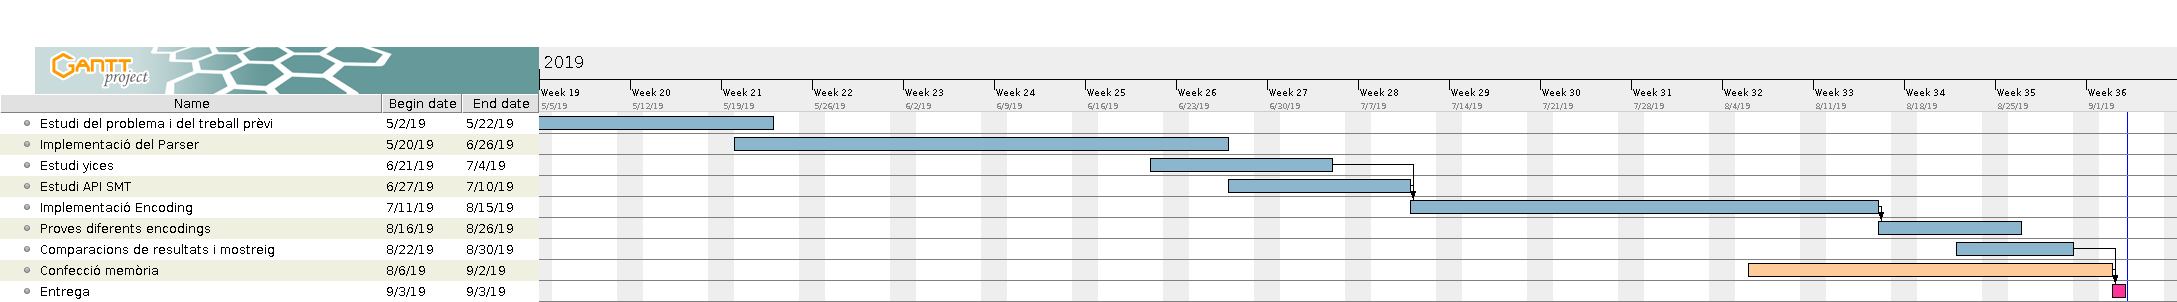
\includegraphics[angle=90,origin=c,height=0.58\textheight]{Diagrames/gantt2.png} 
    \caption{Diagrama de Gantt amb el treball realitzat en el projecte}
    \label{fig:Gantt2}
  \end{figure}
 



  
  

  % Brazil Instance 4 is a real problem, collected in the year 2000 by M.J.F. Souza, at the public school Dom Silvério, located in Mariana, Minas Gerais, Brasil. This instance corresponds to the morning shift at this school. It was provided in XHSTT format by Haroldo Santos. Haroldo's solution can be found on page 69 (Appendix B) of his PhD thesis.

  %razil Instance 6 is a real problem, collected in the year 2000, at the public school Dom Silvério, located in Mariana, Minas Gerais, Brasil. This instance corresponds to the evening shift at this school. In the work of M.J.F. Souza et al, it corresponds to data set DS00N. It was provided in XHSTT by Haroldo Santos.



  \chapter{Treball futur}

  En primer lloc seria interessant afegir encodings de les diferents restriccions del problema que no suporta actualment el generador d'horaris, posat que ens hem centrat en un sub-conjunt de les instàncies disponibles, les que tenen els recursos assignats prèviament.

  Es podrien explorar els paradigmes de SMT i intentar codificar el problema amb les diferents teories que té, com ara els BitVectors.

  També es podrien millorar les codificacions i el model en sí per utilitzar menys memòria i sobretot, per intentar aconseguir millors resultats al optimitzar el problema, comparant amb les diferents solucions disponibles per a cada instància.

  Pel que fa la optimització, com s'ha vist, no s'han aconseguit els resultats desitjats, per això, s'ha de millorar en general. En particular s'hauria de millorar el mètode de càlcul del cost de violar certes restriccions i s'hauria d'afegir un mètode que calcules un bon \textit{upperbound} per tal de donar un millor punt de partida al intentar optimitzar.

  \nocite{*}
  \chapter{Bibliografía}
  \printbibliography[heading=none]
  \chapter{Manual d'usuari i insta\l.lació}

  \section{Compilació}

  Hi ha un \textit{Makefile} per a poder compilar el projecte. Per fer-ho cal tenir insta\l.lades les llibreries \textit{pugixml}\footnote{\url{https://pugixml.org/}} i \textit{yices2}\footnote{\url{https://yices.csl.sri.com/}}
  
  Per a compilar de forma que s'obtingui el millor rendiment, no cal utilitzar cap paràmetre, però si es vol la versió de depuració, cal ficar el paràmetre \textit{DEBUG:=1}.
  \begin{center}
  \begin{itemize}
    \item Per a compilar normalment: \texttt{make}
    \item Per a compilar amb capacitat de depurar: \texttt{make DEBUG:=1}
  \end{itemize}
  \end{center}

  Això deixa l'executable en la carpeta ./bin/linux sota el nom \textit{hstt2smt}


  \section{Ús}
  
  El resultat de compilar com s'ha vist anteriorment, és un executable amb els següents paràmetres rellevants:
  \begin{itemize}
    \item fitxer: instància XHSTT que es vol resoldre.
    \item \texttt{-ub, --upper-bound}: per indicar un upper-bound al resoldre
    \item \texttt{--use-assumptions=0}: paràmetre heretat de la API SMT, s'ha de ficar a 0, perquè no s'han implementat assumpcions.
    \item \texttt{-o, --optimizer}: permet triar l'optimitzador a utilitzar, si es tria \textit{check} no optimitza. Opcions: \texttt{check, ub, bu, dico, native}
  \end{itemize}

  Per exemple, per a resoldre la primera instància de Brazil, anomenada \textit{BrazilInstance1.xml} que es troba en la carpeta \textit{Instances}, es pot fer (l'ordre dels paràmetres no importa):

  \begin{center}
    \texttt{./bin/linux/hstt2smt instances/BrazilInstance1.xml --use-assumptions=0 -o=check}
  \end{center}
  
  \end{document}